
%!TEX TS-program = pdflatex
%!TEX encoding = UTF-8 Unicode

%This is a simple template for a LaTeX document using the "article" class.
%See "book", "report", "letter" for other types of document.

\documentclass[12pt]{article} % use larger type; default would be 10pt

\usepackage[utf8]{inputenc} % set input encoding (not needed with XeLaTeX)

%%% Examples of Article customizations
%These packages are optional, depending whether you want the features they provide.
%See the LaTeX Companion or other references for full information.

%%% PAGE DIMENSIONS
\usepackage{geometry} % to change the page dimensions
\geometry{a4paper} % or letterpaper (US) or a5paper or....
%\geometry{margins=2in} % for example, change the margins to 2 inches all round
%\geometry{landscape} % set up the page for landscape
%read geometry.pdf for detailed page layout information

\usepackage{graphicx} % support the \includegraphics command and options
%\usepackage[parfill]{parskip} % Activate to begin paragraphs with an empty line rather than an indent

%%% PACKAGES
\usepackage{booktabs} % for much better looking tables
\usepackage{array} % for better arrays (eg matrices) in maths
\usepackage{paralist} % very flexible & customisable lists (eg. enumerate/itemize, etc.)
\usepackage{verbatim} % adds environment for commenting out blocks of text & for better verbatim
\usepackage{spverbatim} % adds environment for commenting out blocks of text & for better verbatim
\usepackage{subfig} % make it possible to include more than one captioned figure/table in a single float
% These packages are all incorporated in the memoir class to one degree or another...
\usepackage{listings}

%%%%%%%%%%%%%%%%%%%%%%%%%%%%%%%
%%%%%%%%%%%%%%%%%%%%%%%%%%%%%%%
%%%%%%%%%%%%%%%%%%%%%%%%%%%%%%%
\usepackage{amsmath} % AMS Math Package
\usepackage{amsthm} % Theorem Formatting
\usepackage{amssymb}	% Math symbols such as \mathbb
\usepackage{graphicx} % Allows for eps images
\usepackage{multicol} % Allows for multiple columns
\renewcommand{\labelenumi}{(\alph{enumi})} % Use letters for enumerate
% \DeclareMathOperator{\Sample}{Sample}
\let\vaccent=\v % rename builtin command \v{} to \vaccent{}
\renewcommand{\v}[1]{\ensuremath{\mathbf{#1}}} % for vectors
\newcommand{\gv}[1]{\ensuremath{\mbox{\boldmath$ #1 $}}} 
% for vectors of Greek letters
\newcommand{\uv}[1]{\ensuremath{\mathbf{\hat{#1}}}} % for unit vector
\newcommand{\abs}[1]{\left| #1 \right|} % for absolute value
\newcommand{\avg}[1]{\left< #1 \right>} % for average
\let\underdot=\d % rename builtin command \d{} to \underdot{}
\renewcommand{\d}[2]{\frac{d #1}{d #2}} % for derivatives
\newcommand{\dd}[2]{\frac{d^2 #1}{d #2^2}} % for double derivatives
\newcommand{\pd}[2]{\frac{\partial #1}{\partial #2}} 
% for partial derivatives
\newcommand{\pdd}[2]{\frac{\partial^2 #1}{\partial #2^2}} 
% for double partial derivatives
\newcommand{\pdc}[3]{\left( \frac{\partial #1}{\partial #2}
 \right)_{#3}} % for thermodynamic partial derivatives
\newcommand{\ket}[1]{\left| #1 \right>} % for Dirac bras
\newcommand{\bra}[1]{\left< #1 \right|} % for Dirac kets
\newcommand{\braket}[2]{\left< #1 \vphantom{#2} \right|
 \left. #2 \vphantom{#1} \right>} % for Dirac brackets
\newcommand{\matrixel}[3]{\left< #1 \vphantom{#2#3} \right|
 #2 \left| #3 \vphantom{#1#2} \right>} % for Dirac matrix elements
\newcommand{\grad}[1]{\gv{\nabla} #1} % for gradient
\let\divsymb=\div % rename builtin command \div to \divsymb
\renewcommand{\div}[1]{\gv{\nabla} \cdot #1} % for divergence
\newcommand{\curl}[1]{\gv{\nabla} \times #1} % for curl
\let\baraccent=\= % rename builtin command \= to \baraccent
\renewcommand{\=}[1]{\stackrel{#1}{=}} % for putting numbers above =
\newtheorem{prop}{Proposition}
\newtheorem{thm}{Theorem}[section]
\newtheorem{lem}[thm]{Lemma}
\theoremstyle{definition}
\newtheorem{dfn}{Definition}
\theoremstyle{remark}
\newtheorem*{rmk}{Remark}
%%%%%%%%%%%%%%%%%%%%%%%%%%%%%%%
%%%%%%%%%%%%%%%%%%%%%%%%%%%%%%%
%%%%%%%%%%%%%%%%%%%%%%%%%%%%%%%

\usepackage{wrapfig} %Para insertar imágenes dentro del texto
\usepackage{graphicx} %Para insertar imágenes
\usepackage{appendix}  %Para poner un apéndice
\usepackage{hyperref}



%%% HEADERS & FOOTERS
\usepackage{fancyhdr} % This should be set AFTER setting up the page geometry
\pagestyle{fancy} % options: empty , plain , fancy
\renewcommand{\headrulewidth}{0pt} % customise the layout...
\lhead{}\chead{}\rhead{}
\lfoot{}\cfoot{\thepage}\rfoot{}

%%% SECTION TITLE APPEARANCE
\usepackage{sectsty}
\allsectionsfont{\sffamily\mdseries\upshape} % (See the fntguide.pdf for font help)
% (This matches ConTeXt defaults)

%%% ToC (table of contents) APPEARANCE
\usepackage[nottoc,notlof,notlot]{tocbibind} % Put the bibliography in the ToC
\usepackage[titles,subfigure]{tocloft} % Alter the style of the Table of Contents
\renewcommand{\cftsecfont}{\rmfamily\mdseries\upshape}
\renewcommand{\cftsecpagefont}{\rmfamily\mdseries\upshape} % No bold!

%Para poder elegir el tamaño de los márgenes
\usepackage{anysize}

%\input{header.tex}

%%%Para poner en castellano los titulos de las secciones
\renewcommand{\contentsname}{Contenidos}
\renewcommand{\listfigurename}{Figuras}
\renewcommand{\listtablename}{Tablas}
\renewcommand{\refname}{Bibliograf\'ia}
\renewcommand{\tablename}{Tabla}
\renewcommand{\figurename}{Figura}
\renewcommand{\appendixpagename}{Apéndices} 
%%% END Article customizations

%%% The "real" document content comes below...

%Los siguientes paquetes son para que no corte las palabras
\pretolerance=2000
\tolerance=3000 


\usepackage{geometry}
 \geometry{
 a4paper,
 left=15mm,
 right=10mm,
 top=20mm,
 bottom=20mm,
 }


%AQUI EMPIEZAN LAS MODIFICACIONES DEPENDIENDO DEL TRABAJO


\begin{document}

\section*{Condiciones iniciales}

\paragraph{Unidades}
Se usa un sistema de unidades en cual G = 1, [M] = ...  [l] = 1kpc $\implies$ [v]= ... [t] = ....


\subsection*{los modelos individuales}

\begin{description}
\item modelo elíptico obtenido con isomodr4 (...) 50000 particulas(10000 en el bulbo y 40000 en el halo)
\item modelo con disco obtenido con ... (...) 20000 particulas (8000 en el disco, 4000 en el bulbo, 8000 en el halo) con masa total = 1
\item el modelos elíptico se escala a una masa total 0.1 (cuando se escalan los modelos el radio se escala también para que se cumpla la relación: $\frac{R_1}{R_2} = \sqrt{\frac{M_1}{M_2}}$). Es mejor escalar el segundo modelo antes de ponerlos en órbita usando \textbf{scale} y no especificando estas relaciones en setorbdat porque parece que no funciona
\item los parámetros que se van a configurar para tree500 en TREEPAR: dt y eps dependen de estos modelos iniciales
\begin{description}
\item Calculamos dt = $\frac{1}{20}\sqrt{\frac{R^3}{M}}$ ,  eps = $0.2 R$ donde R es el radio de media masa y M es la media masa de la parte luminos elijiendo los valores mas pequeños de los 2 modelos
\item
\small
\begin{verbatim}
 nora>> data two.xvp 1
 getmodel>> model :            1
 xvpread>> Reading    70000 particles from model     0.0000 of file :two.xvp                                 
  getmodel:: nbods =   70000.0000       iteration =   300.000000       time =   16.0200100    
 nora>> list head 100 110
   1.00000000    
   5.00000000    
   8000.00000    
   1.02271779E-05
   12000.0000    
   7.43265036E-06
   20000.0000    
   1.10622786E-04
   30000.0000    
   2.49999994E-06
   70000.0000    
 nora>> bodsrange 1 12000
 nora>> Rm 100
#
#FILE two.xvp    MODEL     1                                                    
#PART       1-  12000  VIEW    0.0,   0.0  RMAX 100.0  SLIT  -0.0, 0.0,*****    
#totm =  1.116E-01
#FRM :      0.01     0.02     0.05     0.10     0.20     0.30     0.40     0.50
#Rm  :  2.23E+00 2.29E+00 2.31E+00 2.34E+00 2.40E+00 2.46E+00 2.53E+00 2.59E+00
#FRM :      0.60     0.70     0.80     0.90     0.95     0.98     0.99     1.00
#Rm  :  2.65E+00 2.71E+00 2.77E+00 2.84E+00 2.87E+00 2.89E+00 2.89E+00 1.00E+15
 nora>> bodsrange 30001 40000
 nora>> Rm 100
#
#FILE two.xvp    MODEL     1                                                    
#PART   30001-  40000  VIEW    0.0,   0.0  RMAX 100.0  SLIT  -0.0, 0.0,*****    
#totm =  1.875E-02
#FRM :      0.01     0.02     0.05     0.10     0.20     0.30     0.40     0.50
#Rm  :  1.27E+00 1.48E+00 1.82E+00 1.99E+00 2.30E+00 2.40E+00 2.50E+00 2.60E+00
#FRM :      0.60     0.70     0.80     0.90     0.95     0.98     0.99     1.00
#Rm  :  2.70E+00 2.79E+00 2.89E+00 3.37E+00 3.61E+00 4.16E+00 4.42E+00 1.00E+15

\end{verbatim}

\normalsize
\item $R_1$ = 2.59E+00, $M_1$ = 0.5 * 1.116E-01 $\implies$ $dt_1$ = 0.8822721105537292 y $eps_1$ = 0.518
\item $R_2$ = 2.60E+00, $M_2$ = 0.5 * 1.875E-02 $\implies$ $dt_2$ = 1.5308385501634936 y $eps_2$ = 0.52
\item Con unos valores de dt = 0.8822721105537292 y eps = 0.518 la simulación debería ir bien , pero los valores calculados con estas fórmulas  son valores máximos para estos  parámetros , elijiendo unos valores mas pequeños la simulación tardará más
\item yo elegí dt = 0.1146314 y eps = 0.276

\end{description}

\end{description}

\subsection*{puesta en órbita}
\paragraph{kepler}
\begin{description}
\item  si cambiamos el parámetro de impacto hay que ejecutar de nuevo kepler con la nueva separación
\item el parámetro nsteps de TREEPAR depende del parámetro Period de la salida de kepler: hay que poner un par de veces el periodo hasta el encuentro de los 2 objetos (El número de periodos de la ejecución = nsteps * dt / Period)
\item elegí separacion = 20, 10 y 5
\item separación \textbf{5}
\begin{verbatim}
BINARY:  M2/M1= 0.10000      SEP.(M2)=  5.000     (VR,VT)=( -0.46904,  0.00000)
         AngMom=  0.0000      P.A.(M2)=   0.00      PHI(V)=   0.05    VZ=  0.000
 a=     5.00  r-peri=   0.00  r-apo=  10.00  b=  0.00  e= 1.000  Period=   66.98
            V-peri=999.999V-apo=  0.000V(Now)=  0.469T(peri)=    6.08
 BOUND LINEAR TRAJECTORY -- at Orbital Phase (TRUE ANOMALY) =   -0.0548
\end{verbatim}
\item Period = 66.98, yo elegí nsteps = 4000 lo que corresponde a 6.845 periodos
\item separación \textbf{10}
\begin{verbatim}
 BINARY:  M2/M1= 0.10000      SEP.(M2)= 10.000     (VR,VT)=( -0.33166,  0.00000)
         AngMom=  0.0000      P.A.(M2)=   0.00      PHI(V)=   0.05    VZ=  0.000
 a=    10.00  r-peri=   0.00  r-apo=  20.00  b=  0.00  e= 1.000  Period=  189.45
            V-peri=999.999V-apo=  0.000V(Now)=  0.332T(peri)=   17.21
 BOUND LINEAR TRAJECTORY -- at Orbital Phase (TRUE ANOMALY) =   -0.0548
\end{verbatim}

\item Period = 189.45, yo elegí nsteps = 10000 lo que corresponde a 6.05 periodos

\item separación \textbf{20}
\begin{verbatim}
 BINARY:  M2/M1= 0.10000      SEP.(M2)= 20.000     (VR,VT)=( -0.23452,  0.00000)
         AngMom=  0.0000      P.A.(M2)=   0.00      PHI(V)=   0.05    VZ=  0.000
 a=    20.00  r-peri=   0.00  r-apo=  40.00  b=  0.00  e= 1.000  Period=  535.83
            V-peri=999.999V-apo=  0.000V(Now)=  0.235T(peri)=   48.68
 BOUND LINEAR TRAJECTORY -- at Orbital Phase (TRUE ANOMALY) =   -0.0548

\end{verbatim}

\item Period = 535.83, yo elegí nsteps = 30000 lo que corresponde a 6.41 periodos

\item La órbita es parabólica(Binary Orbital Eccentricity = 1) y por haber elegido  bound linear encounter = yes VT = 0 y por haber elegido Binary Approaching Pericenter = yes VR $<$ 0
Hay que poner los valores de VR obtenidos en este paso en el fichero setorbdat


\end{description}

\paragraph{setorb}

\begin{description}
\item  si cambiamos el angulo del spin de los objetos relativo al plano de la orbita de los 2 (en particular la orientación del spin)
hay que ejecutar de nuevo setorb 

he elegido valores de theta1 = 90, 60, 270, 240

Los modelos están aliniados en la direccion ox

\end{description}
\newpage

\begin{figure}[!ht]
 \centering
 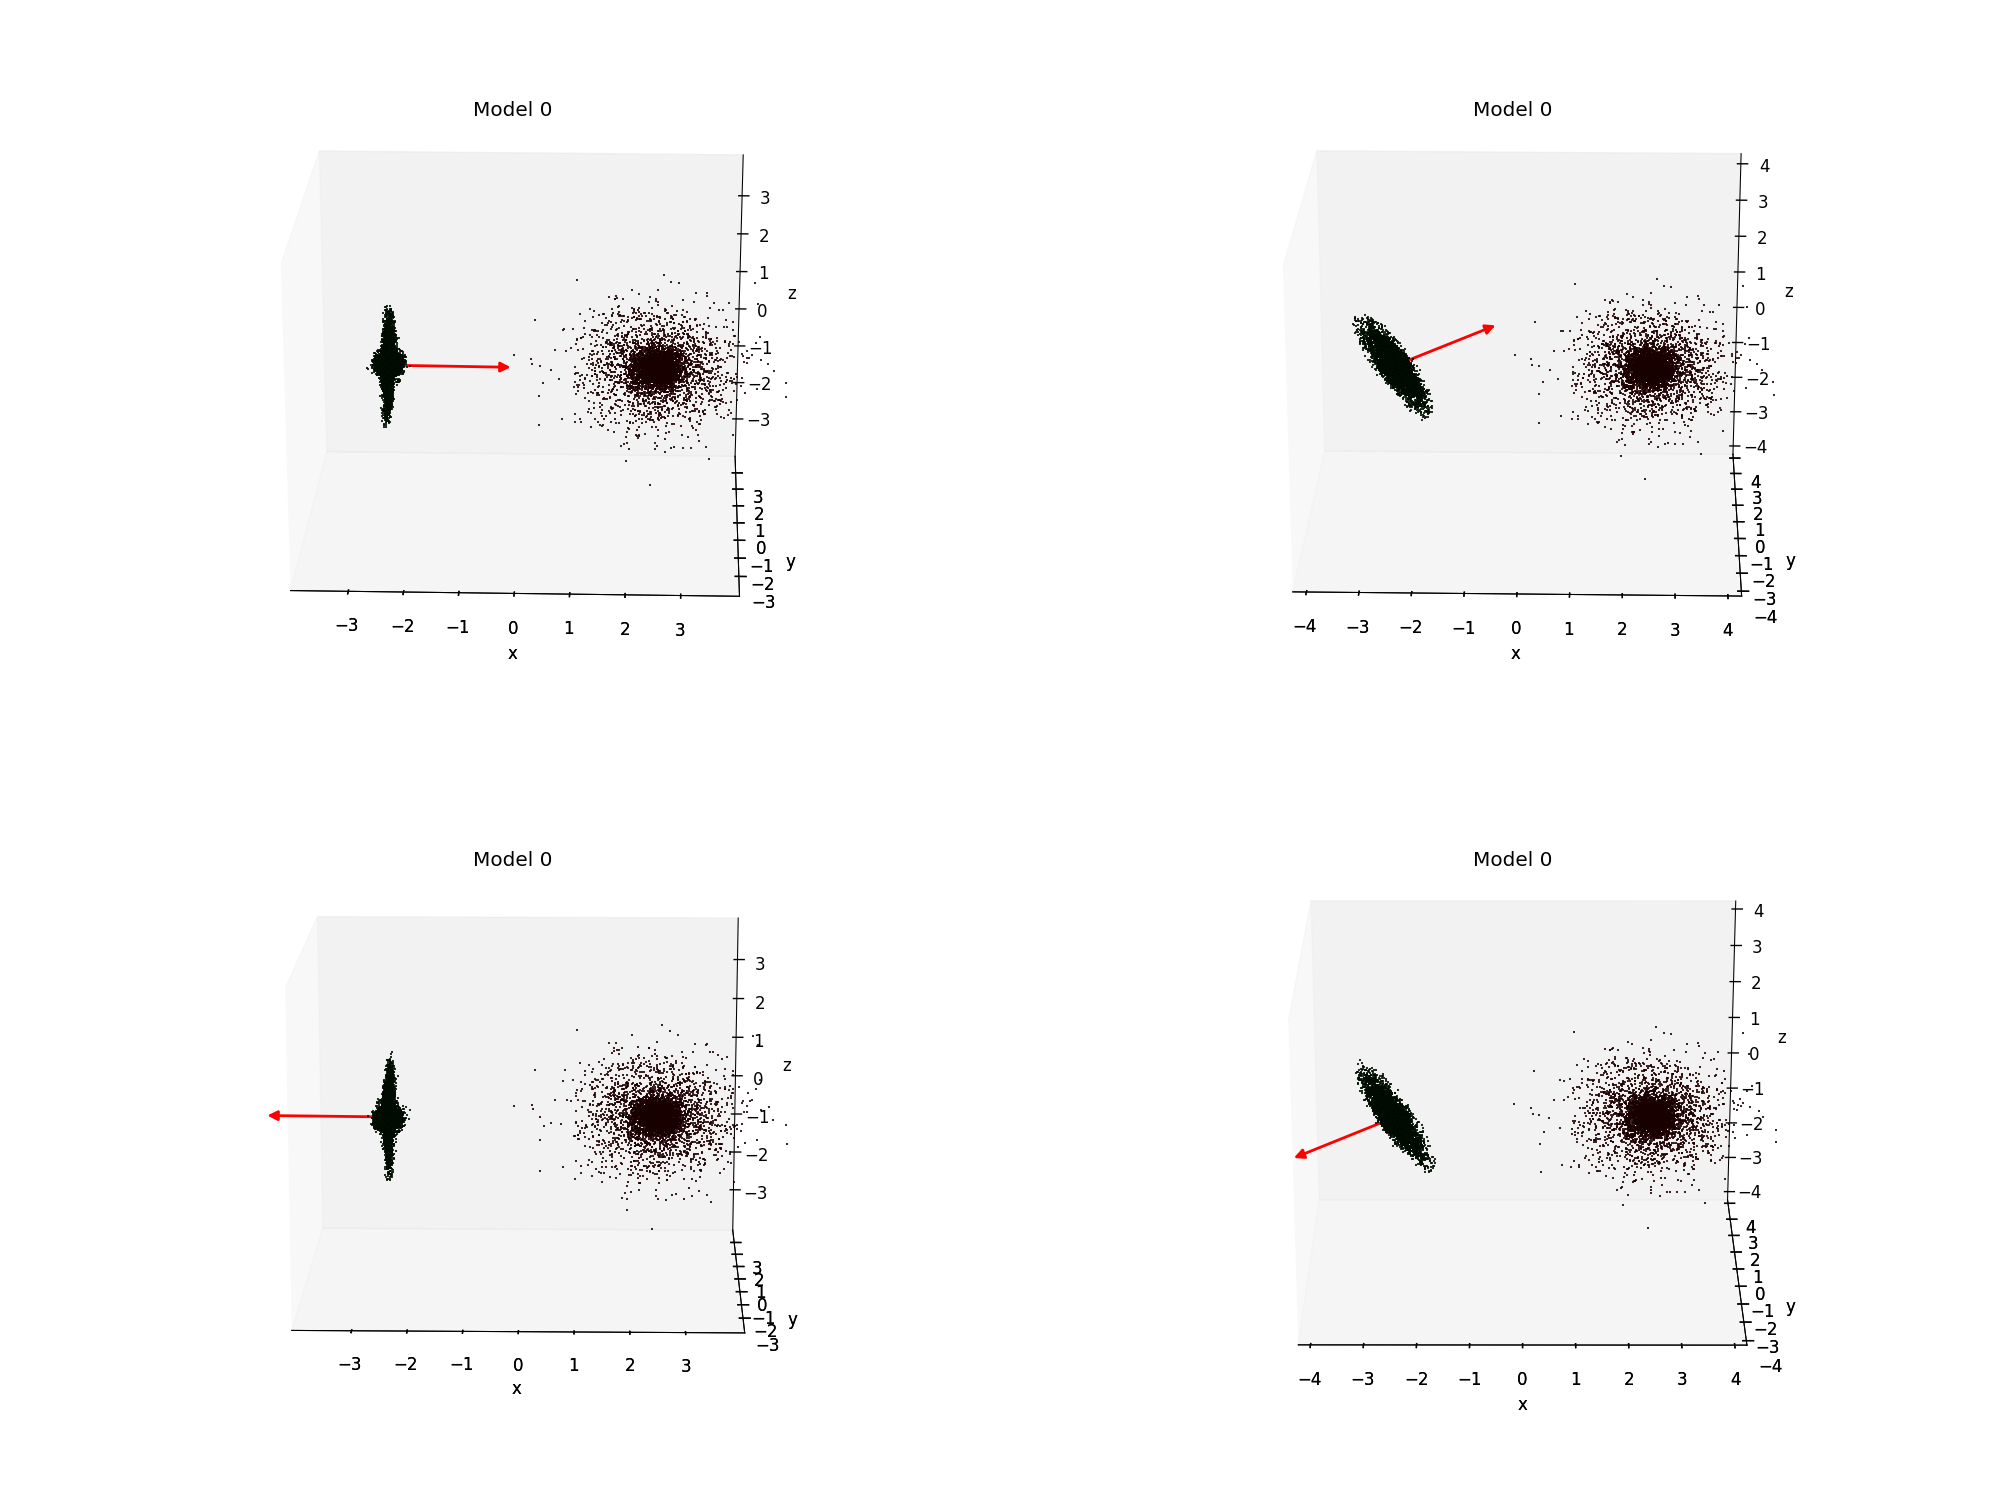
\includegraphics[scale=0.2]{inimod_sep5.png}
 \caption{\emph{Los modelos en el momento inicial(separación = 5), solo la parte luminosa para angulos 90, 60, 270, 240 \\
	Se representa también el vector del momento angular del objeto con disco (el módulo multiplicado por 100) }}
\end{figure}

\begin{figure}[!ht]
 \centering
 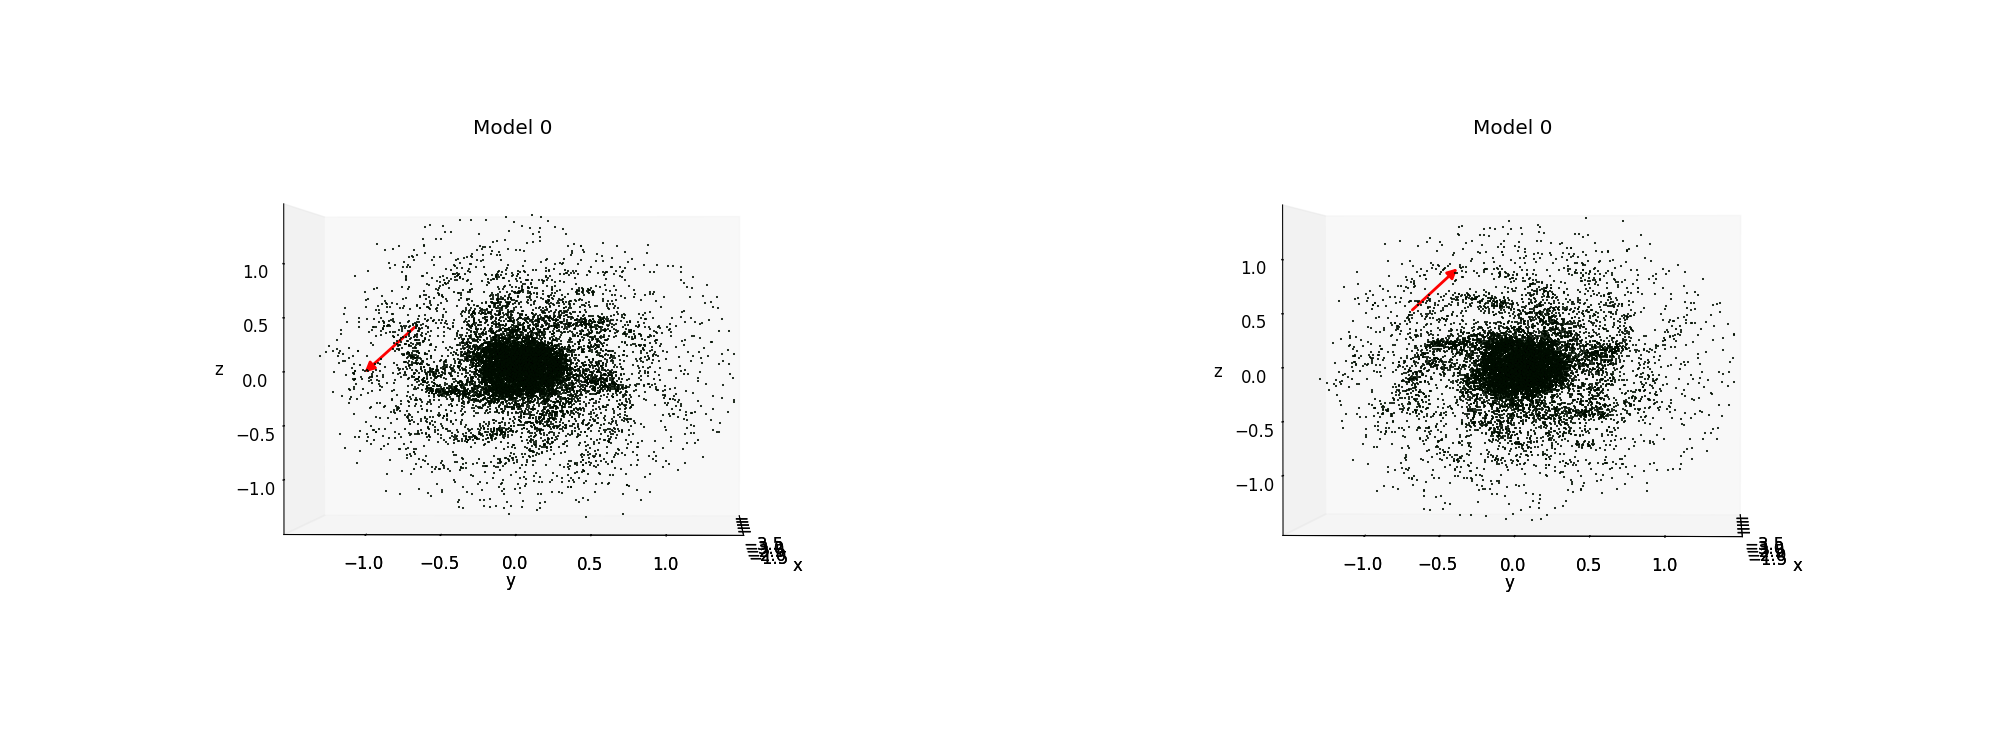
\includegraphics[scale=0.2]{inimoddisco_sep5.png}
 \caption{\emph{El disco y bulbo del primer modelo en el momento inicial visto desde la dirección del otro objeto \\
para los primeros 2 casos (ángulos 90, 60) y para los otros 2 (ángulos 270, 240 - el spin en la otra dirección)}}
\end{figure}





\newpage
\section*{Evolución del modelo}
\paragraph{tree500}



Voy a representar los primeros encuentros (el modelo esférico está atravesando el disco - en caso de la sepración = 5 el primer encuentro pasa en el modelo 1) y el último (modelo 39)
La relación entre el número de modelo y el tiempo es: t = noutbod * dt * numModel = 11.46 *  numModel
(en el caso de la separación = 5 hay 40 modelos con numModel = 0..39)


\begin{figure}[!ht]
 \centering
 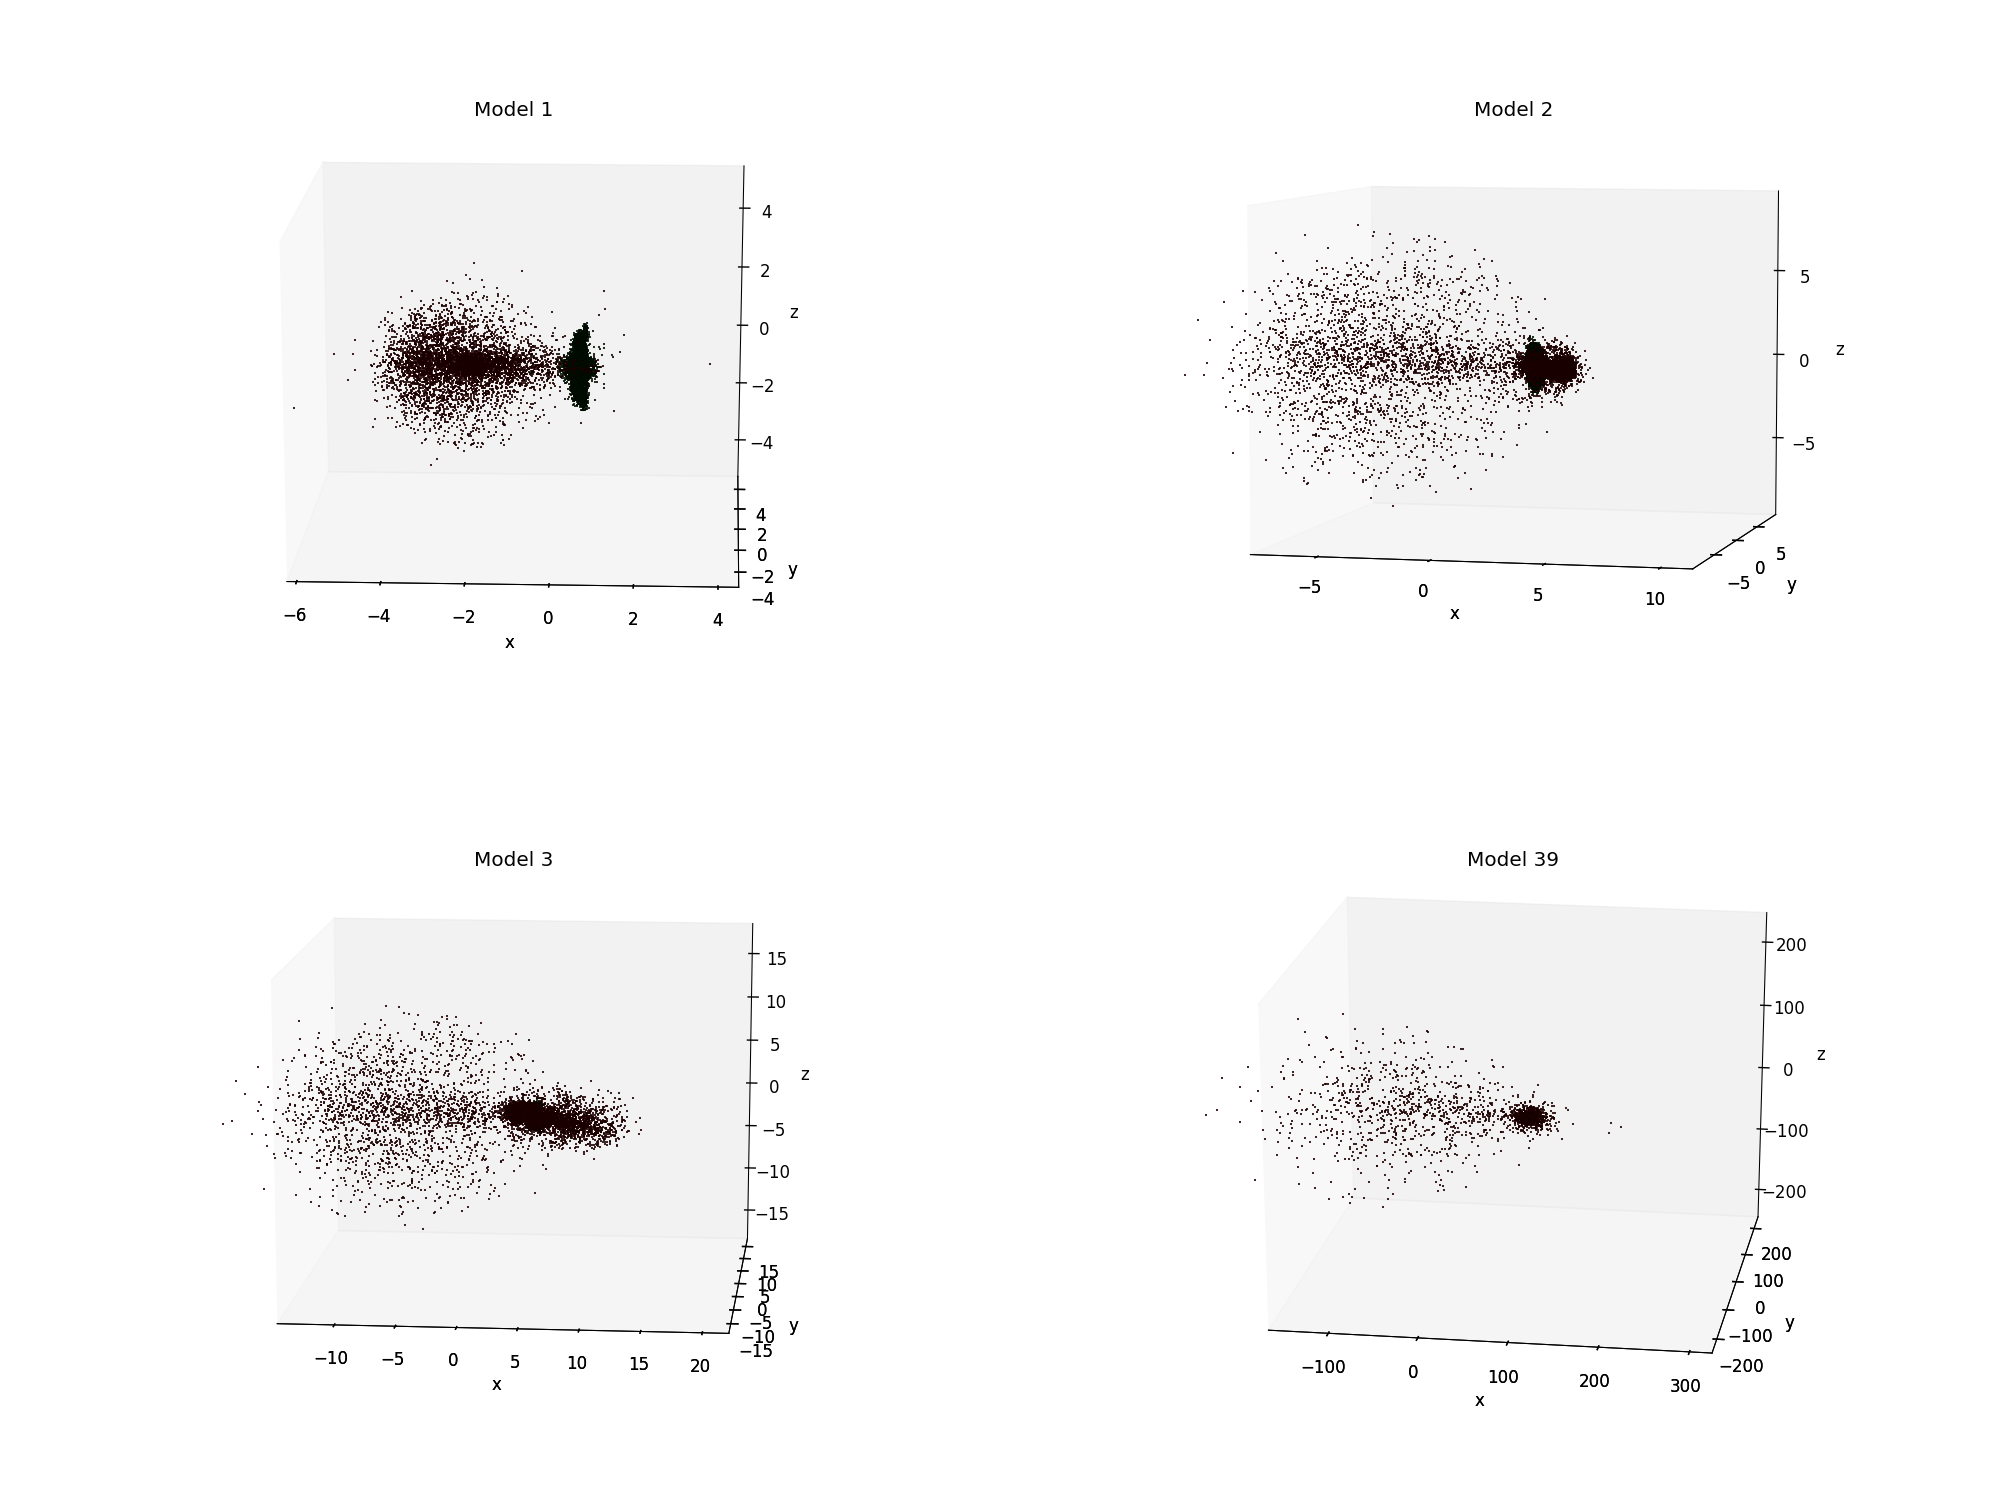
\includegraphics[scale=0.2]{90deg_m_sep5.png}
 \caption{\emph{ ángulo = 90 grados, los 2 objetos(solo parte luminosa) modelo 1,2,3,39 }}
\end{figure}

\begin{figure}[!ht]
 \centering
 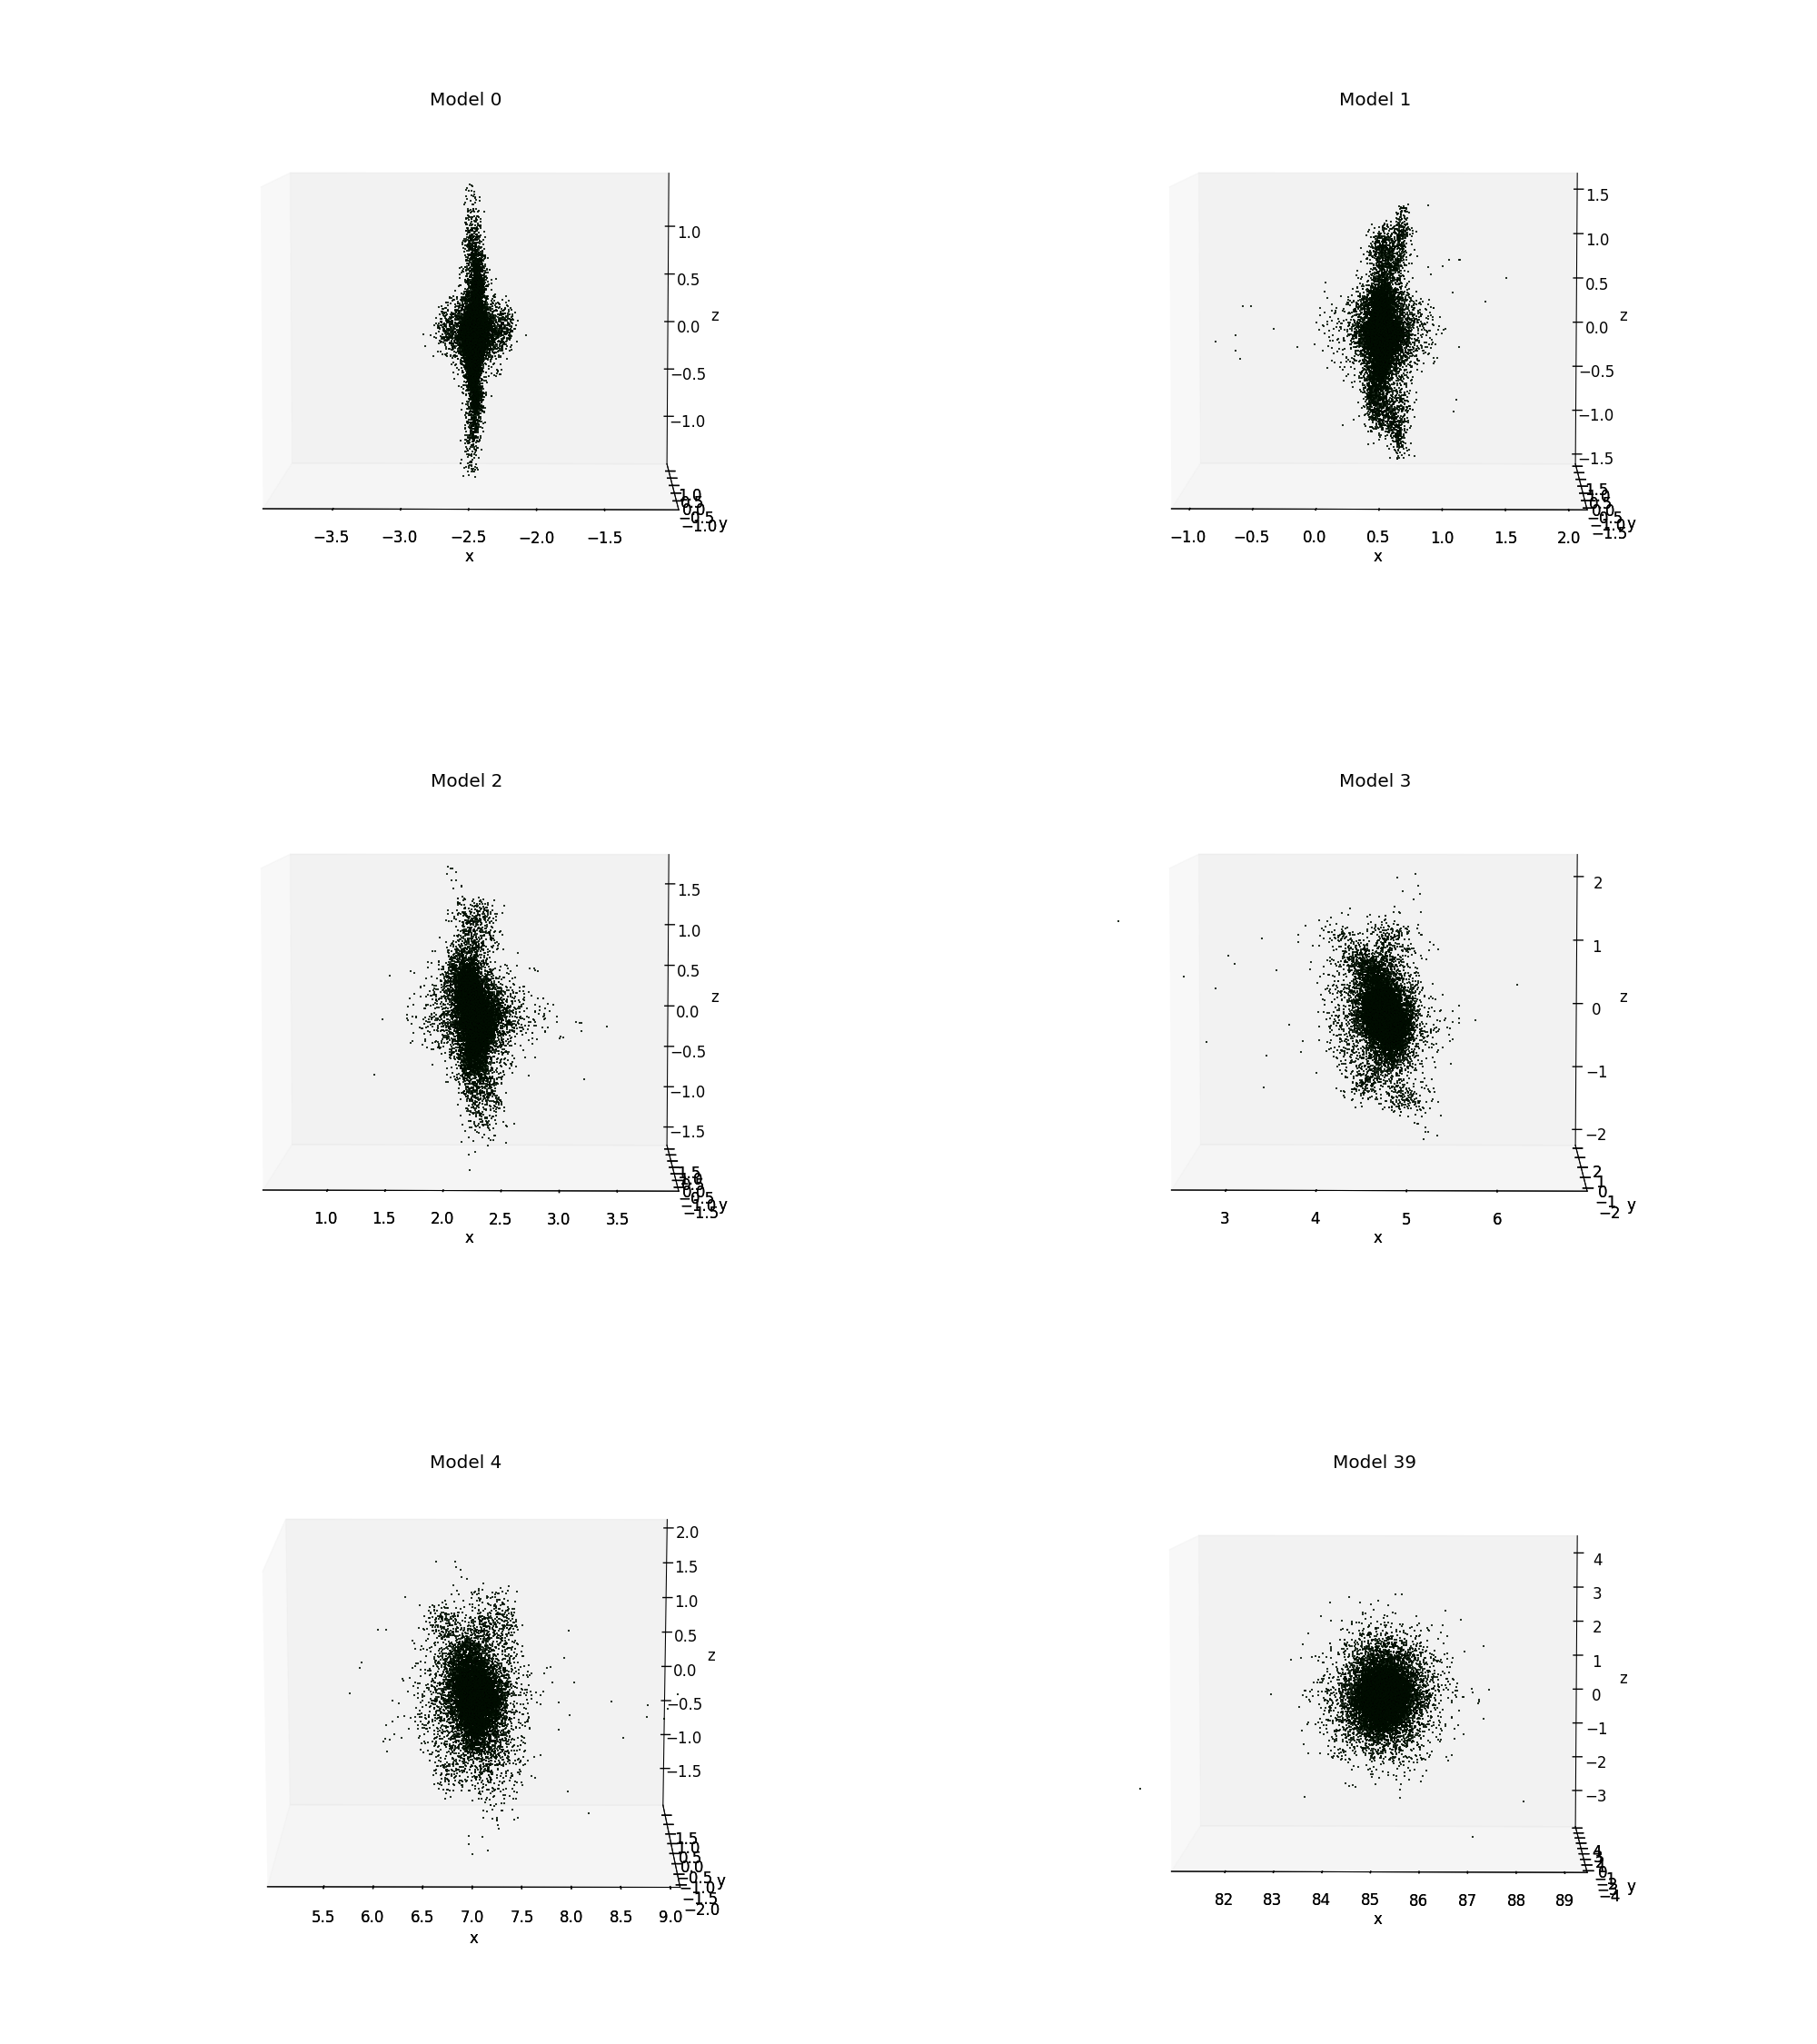
\includegraphics[scale=0.2]{90deg-m-c2y.png}
 \caption{\emph{ ángulo = 90 grados, el objeto con disco visto en la dirección oy(solo parte luminosa) modelo 0,1,2,3,4,39 }}
\end{figure}

\begin{figure}[!ht]
 \centering
 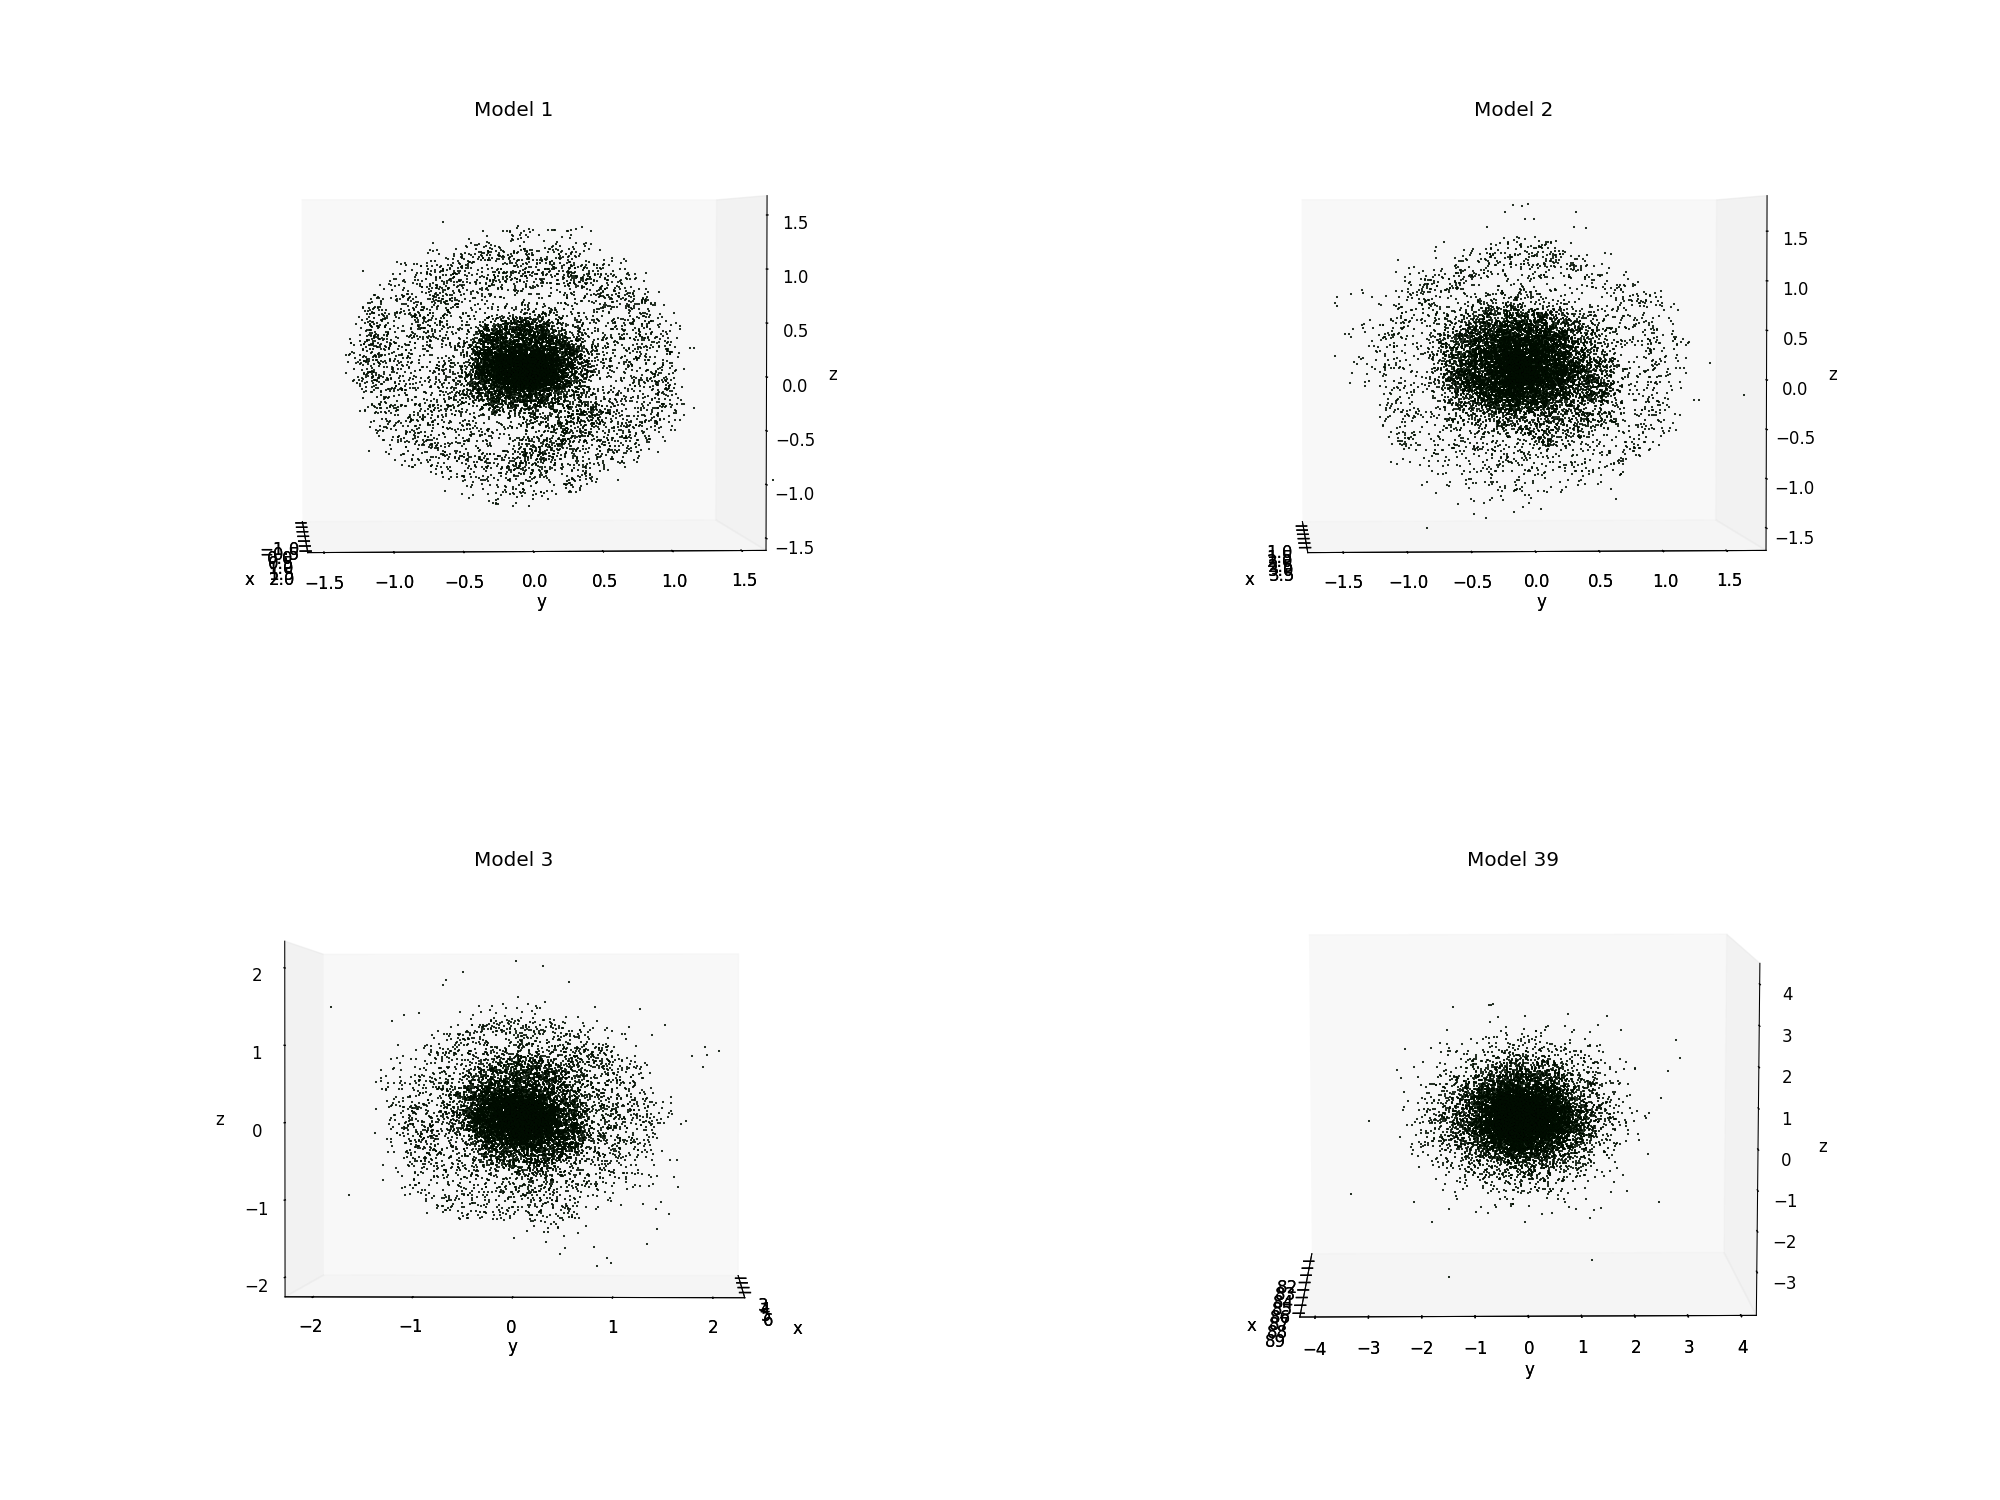
\includegraphics[scale=0.2]{90deg-m-c2.png}
 \caption{\emph{ ángulo = 90 grados, el objeto con disco visto en la dirección ox(solo parte luminosa) modelo 1,2,3,39 }}
\end{figure}


\begin{figure}[!ht]
 \centering
 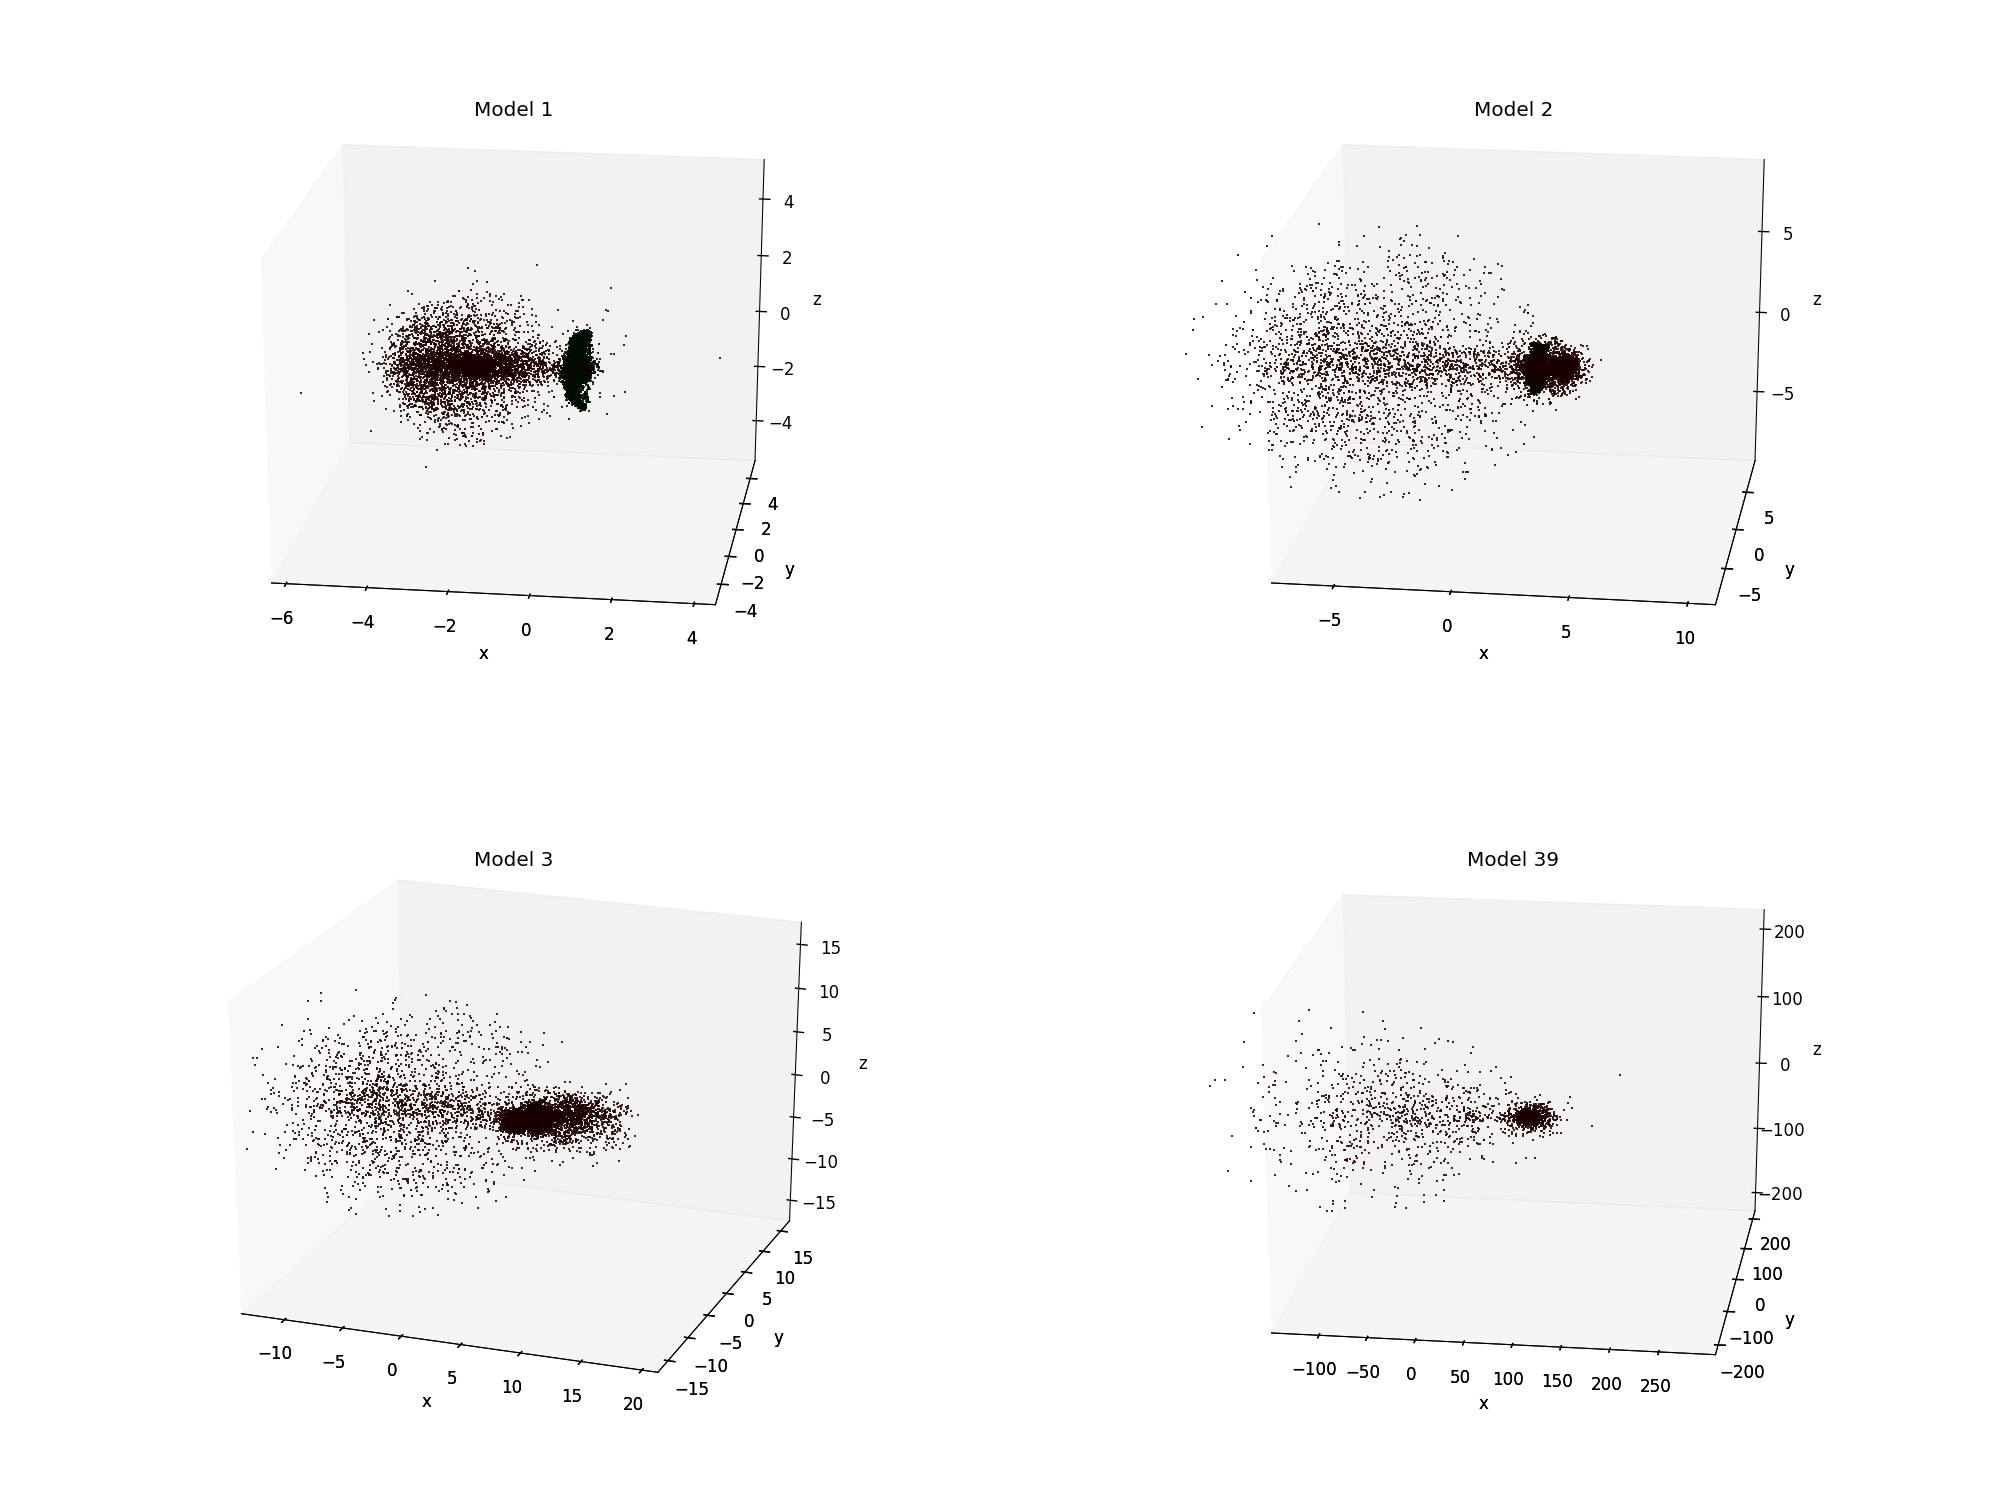
\includegraphics[scale=0.2]{270deg_m_sep5.png}
 \caption{\emph{ ángulo = 270 grados, los 2 objetos(solo parte luminosa) modelo 1,2,3,39 }}
\end{figure}

\begin{figure}[!ht]
 \centering
 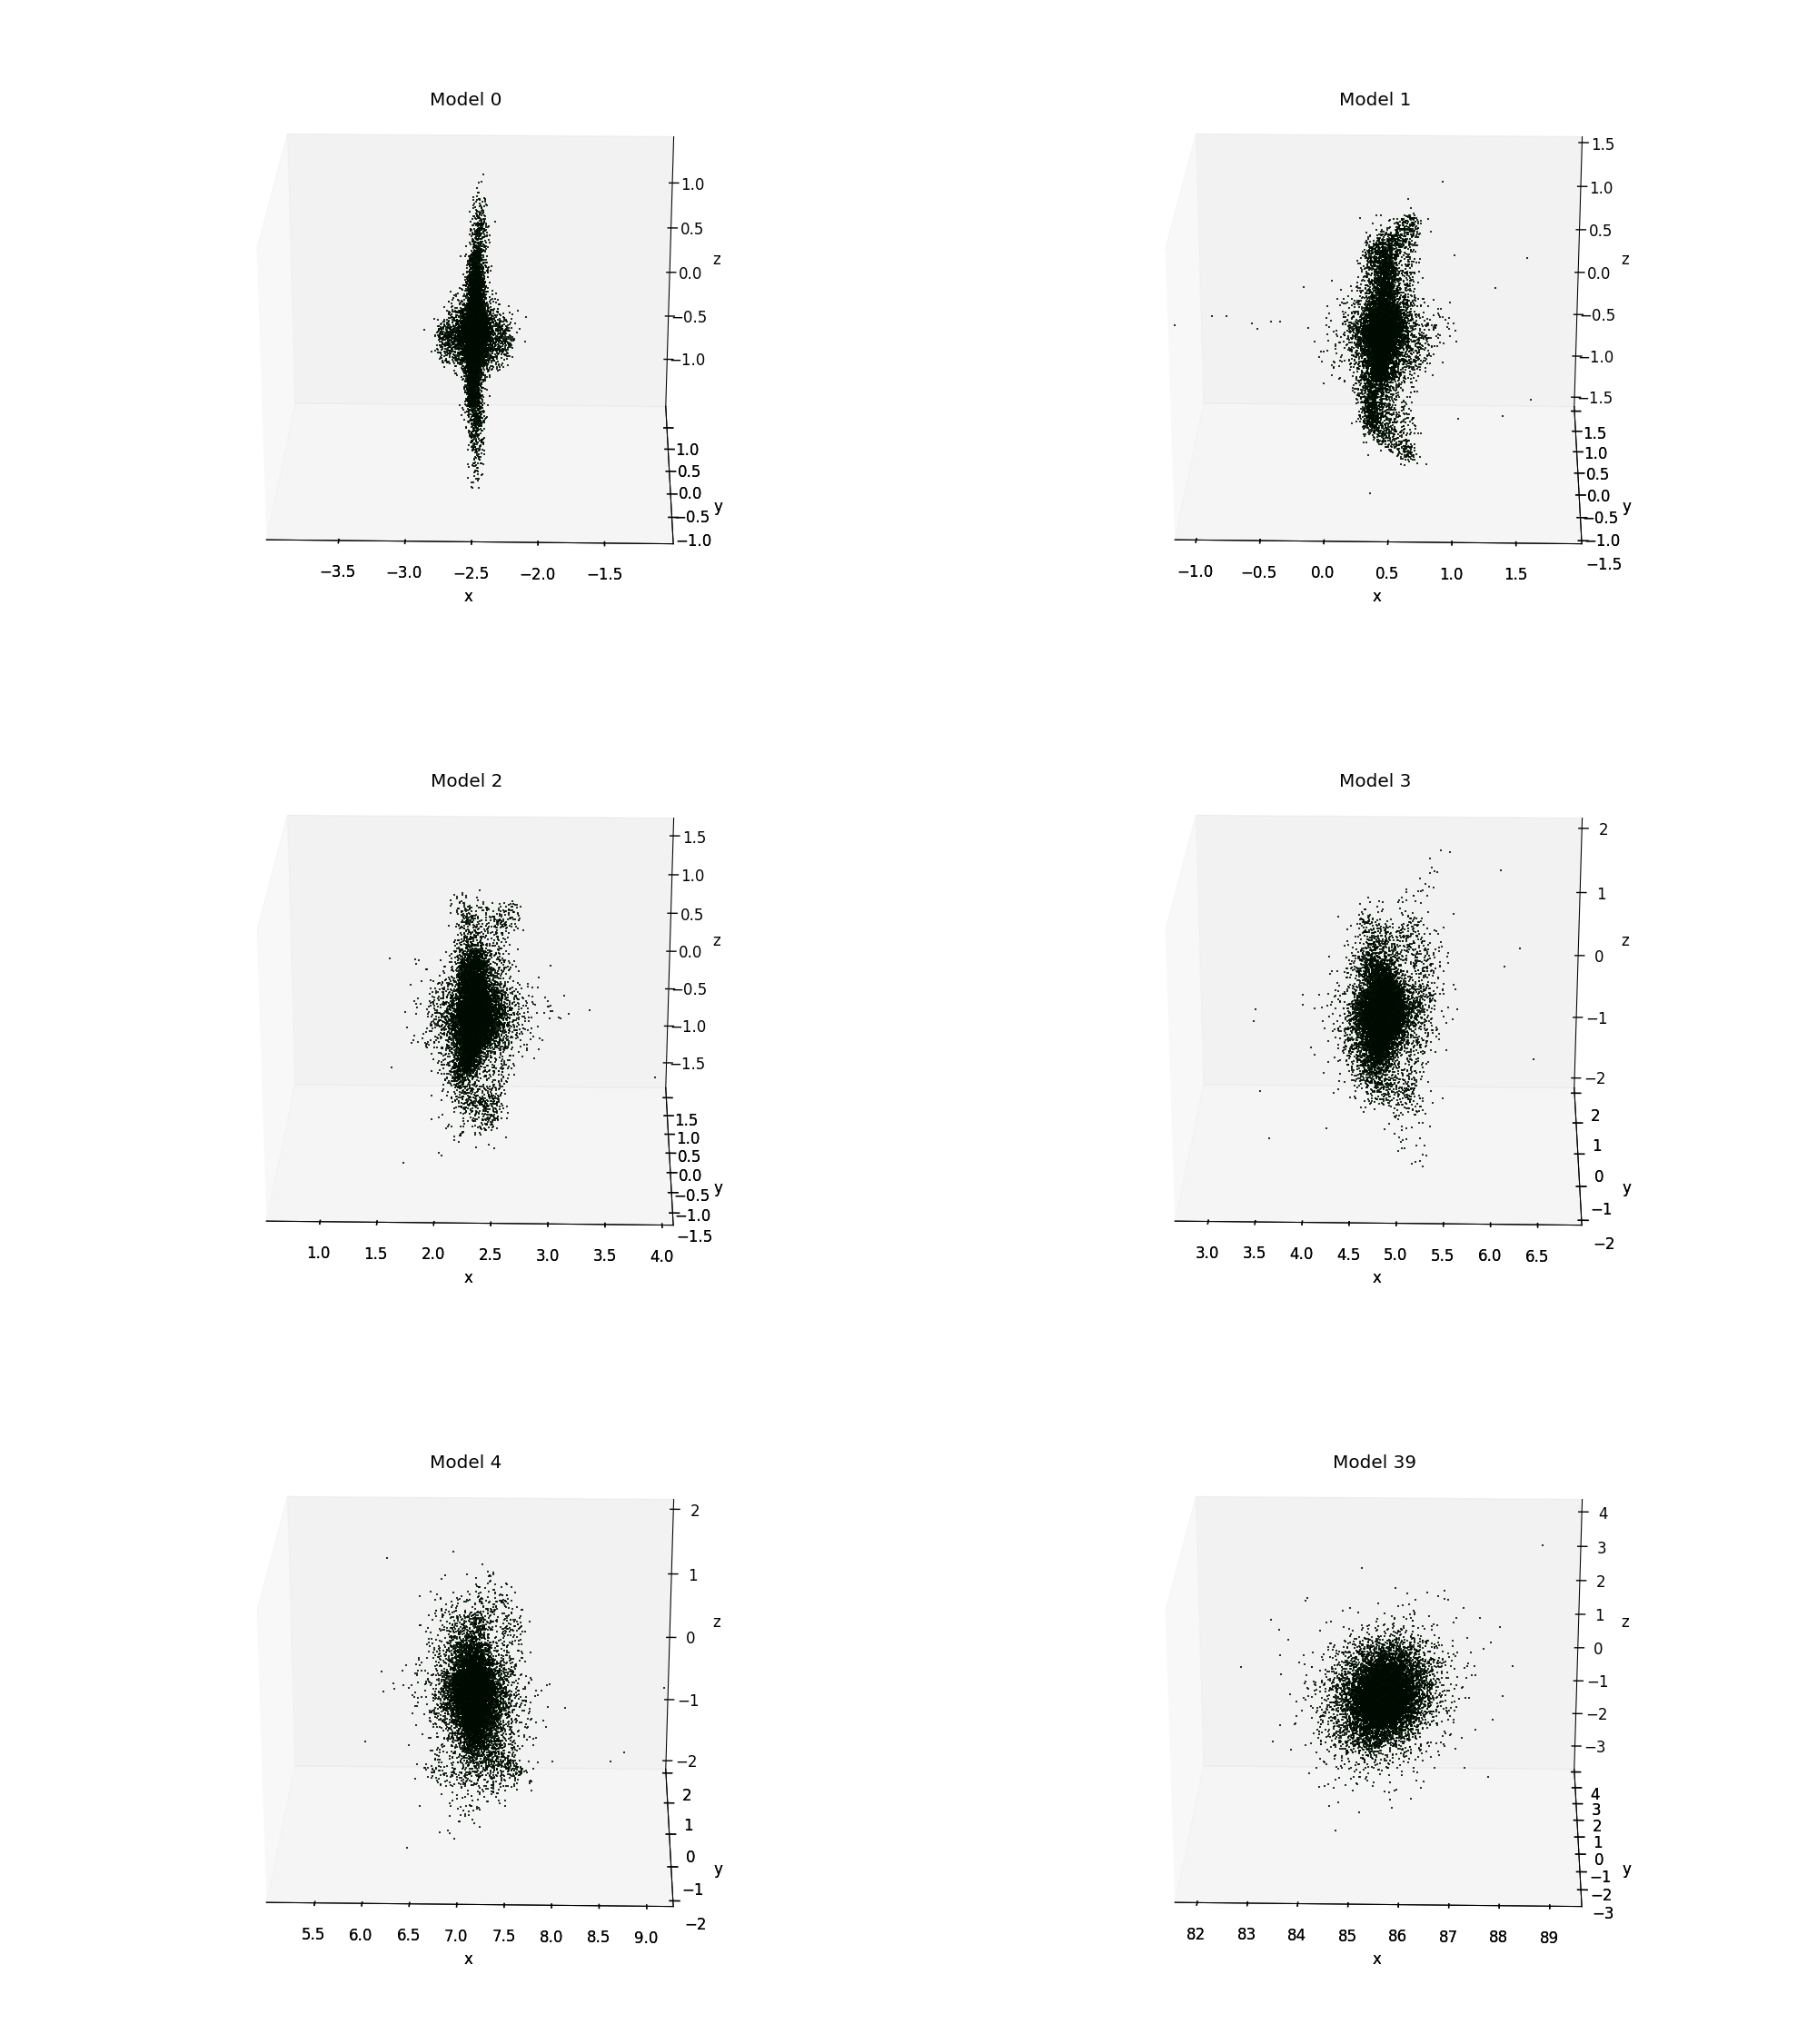
\includegraphics[scale=0.2]{270deg-m-c2y.png}
 \caption{\emph{ ángulo = 270 grados, el objeto con disco visto en la dirección oy(solo parte luminosa) modelo 0,1,2,3,4,39 }}
\end{figure}

\begin{figure}[!ht]
 \centering
 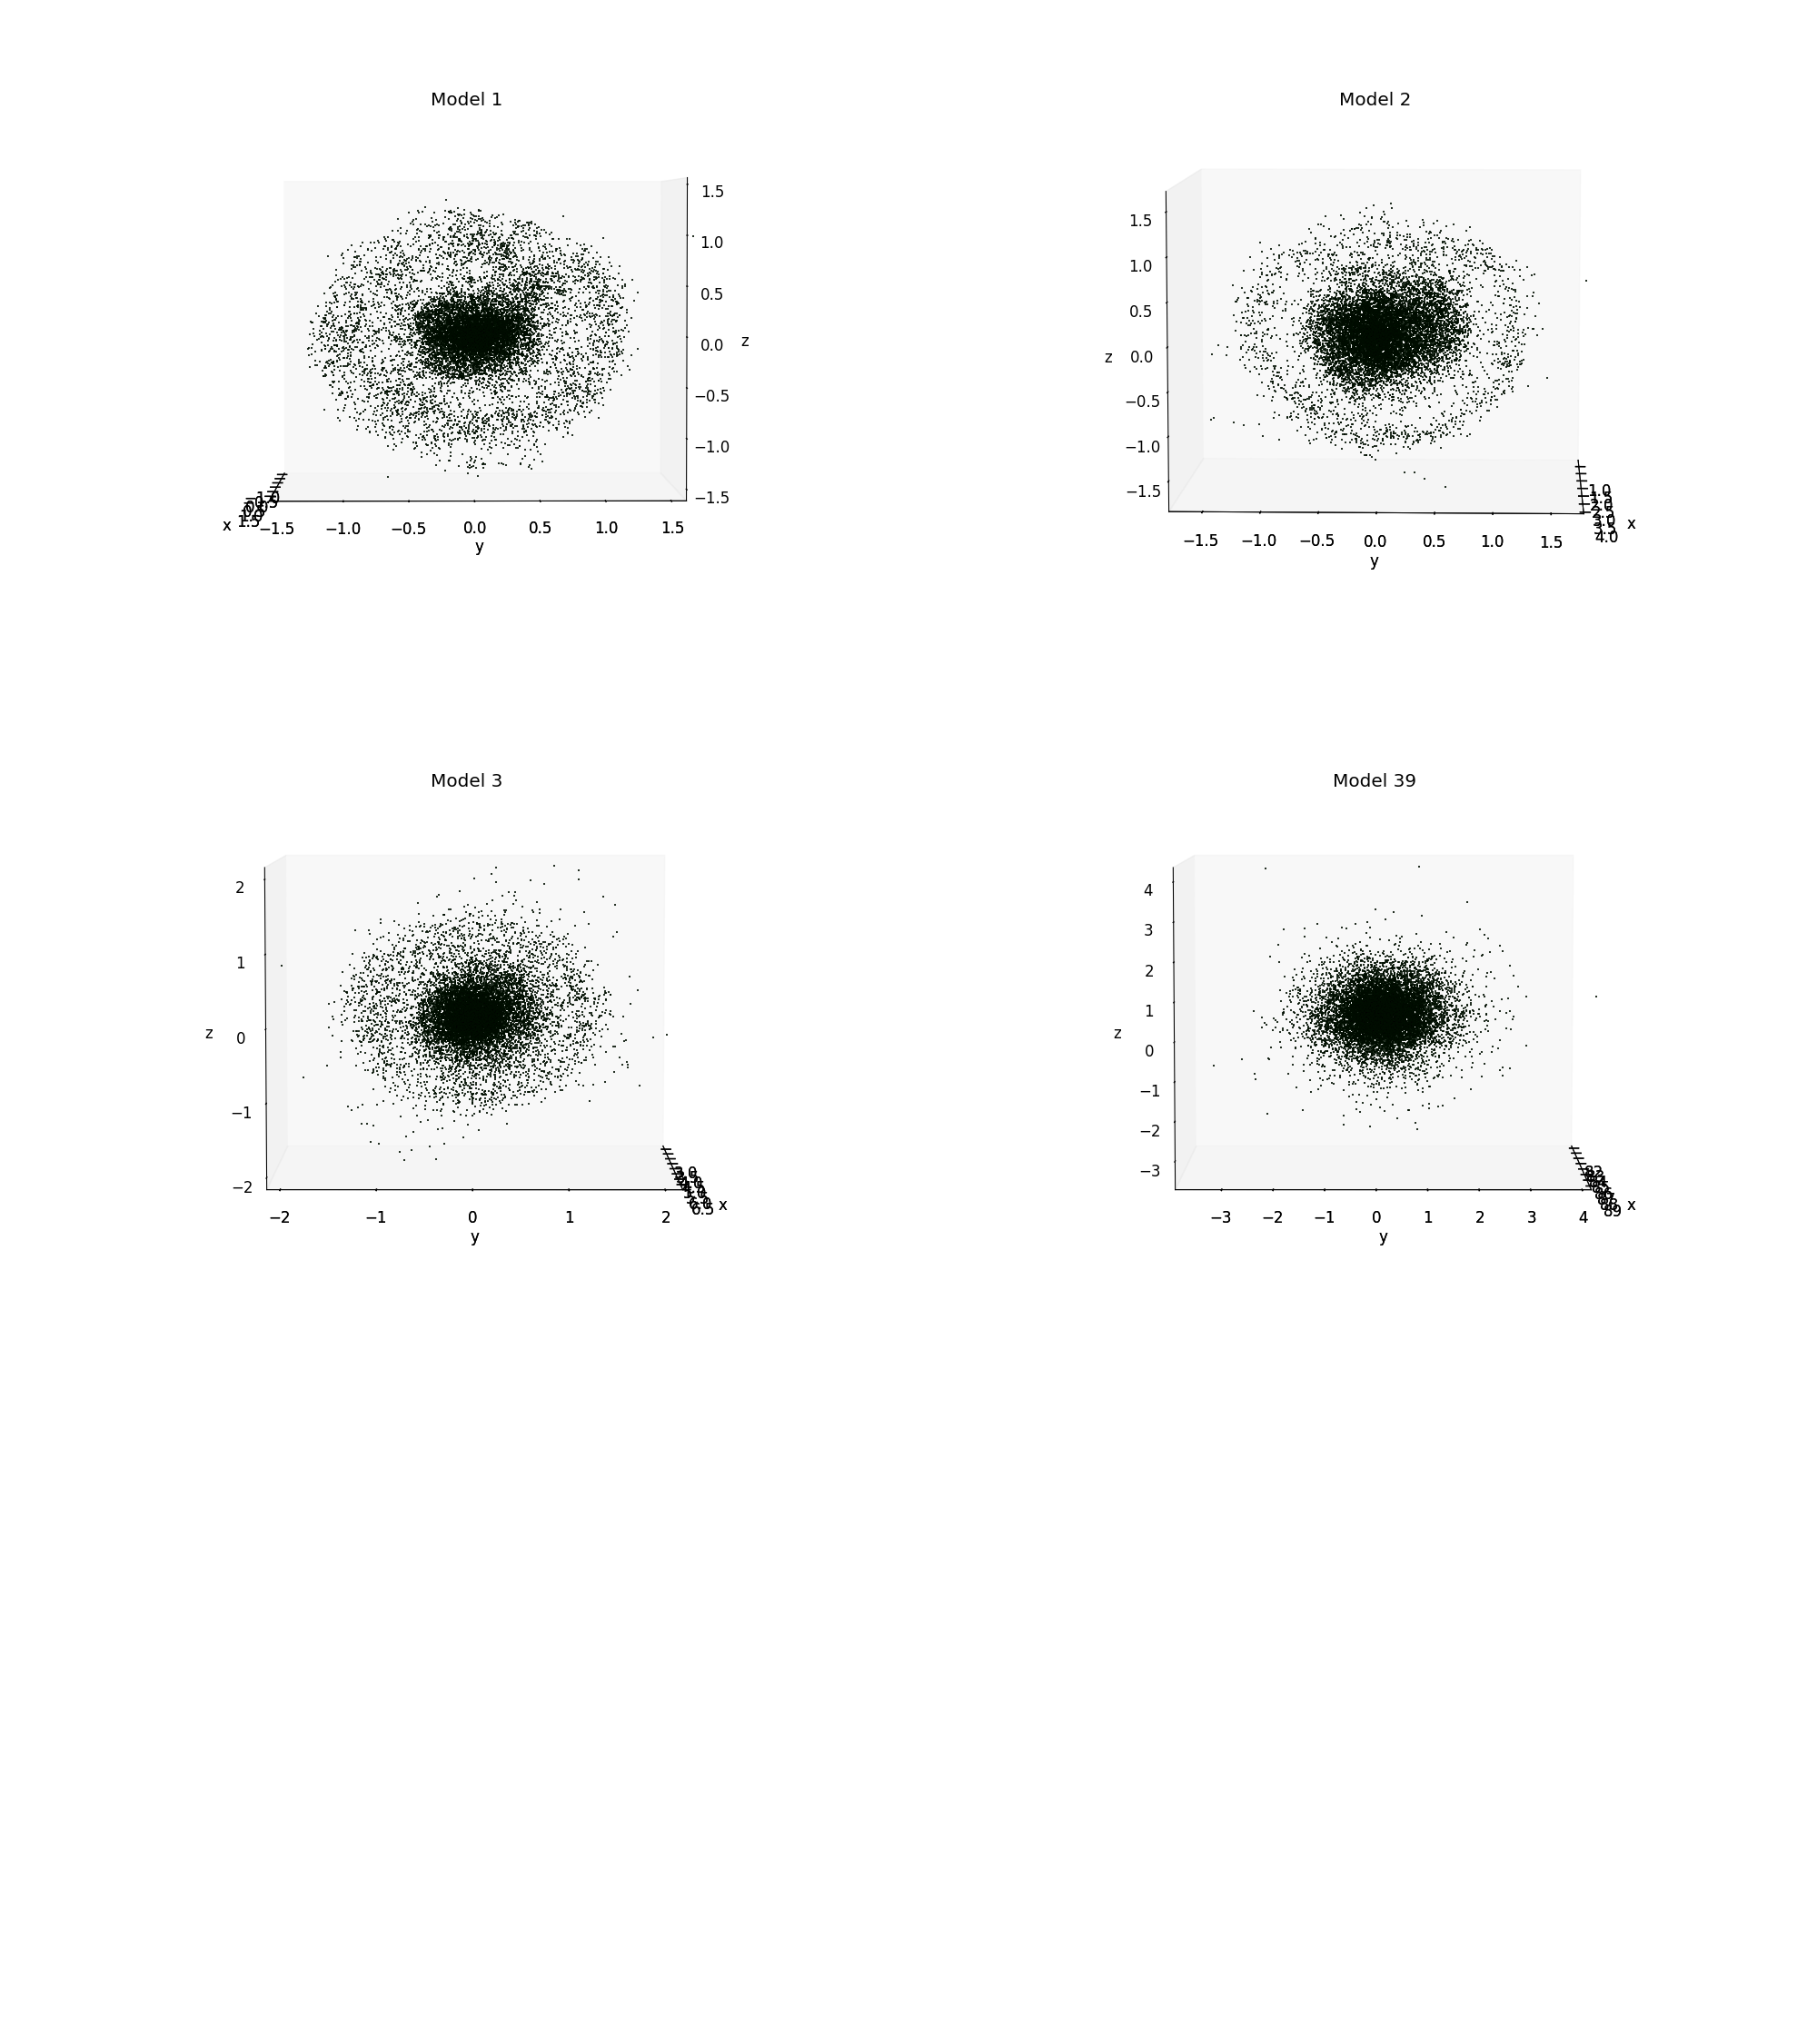
\includegraphics[scale=0.2]{270deg-m-c2.png}
 \caption{\emph{ ángulo = 270 grados, el objeto con disco visto en la dirección ox(solo parte luminosa) modelo 1,2,3,39 }}
\end{figure}


\begin{figure}[!ht]
 \centering
 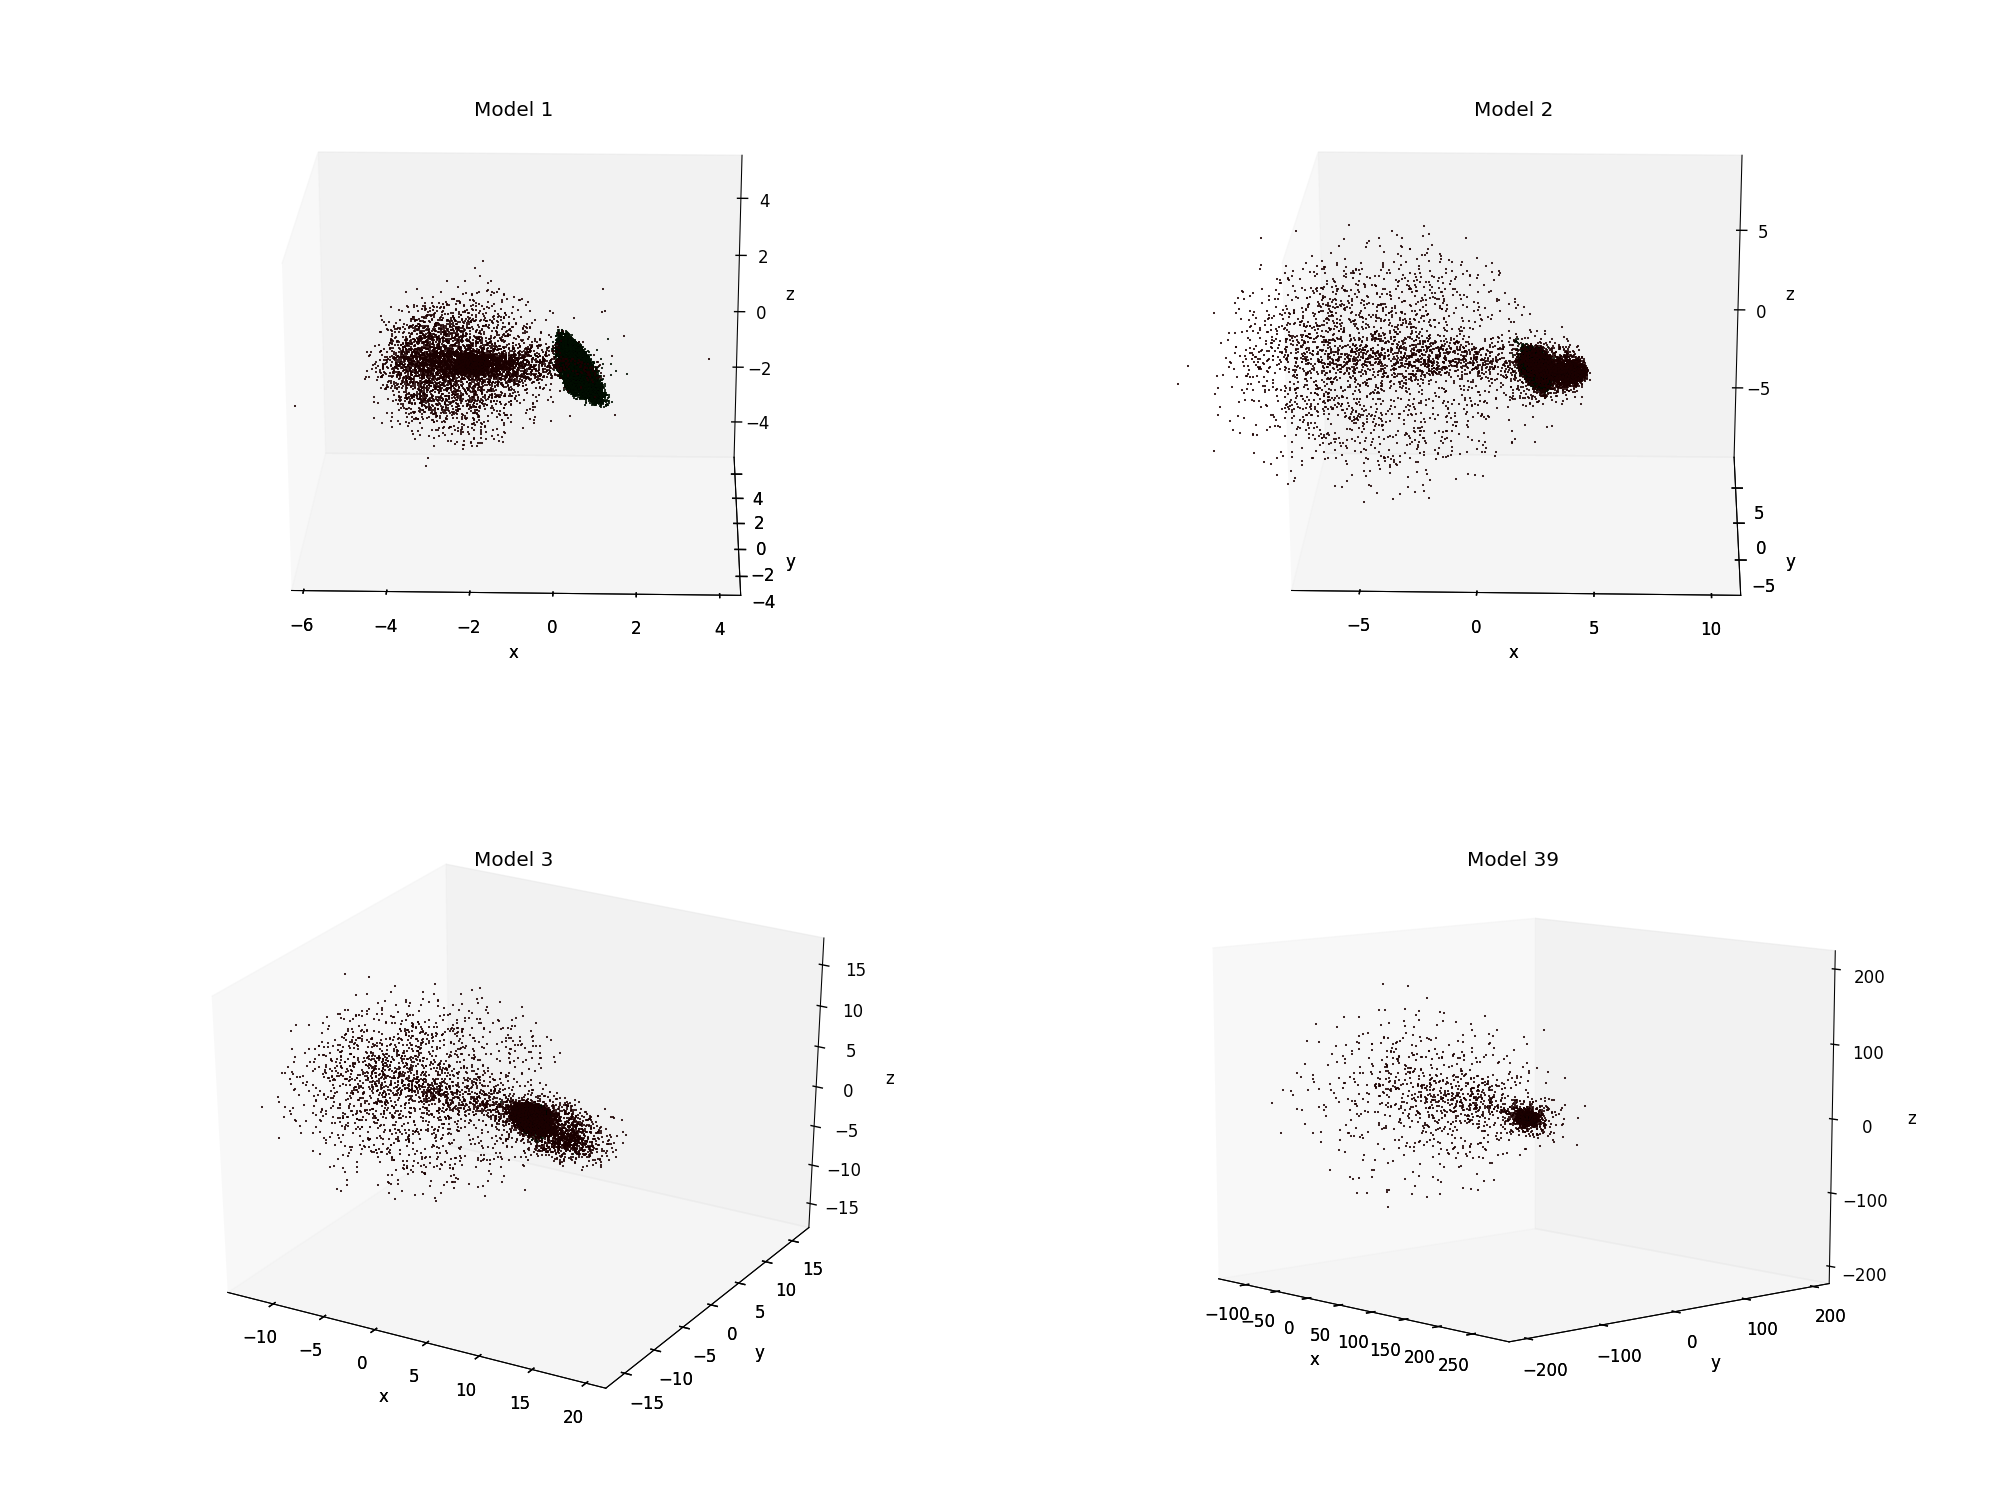
\includegraphics[scale=0.2]{60deg-m.png}
 \caption{\emph{ ángulo = 60 grados, los 2 objetos(solo parte luminosa) modelo 1,2,3,39 }}
\end{figure}

\begin{figure}[!ht]
 \centering
 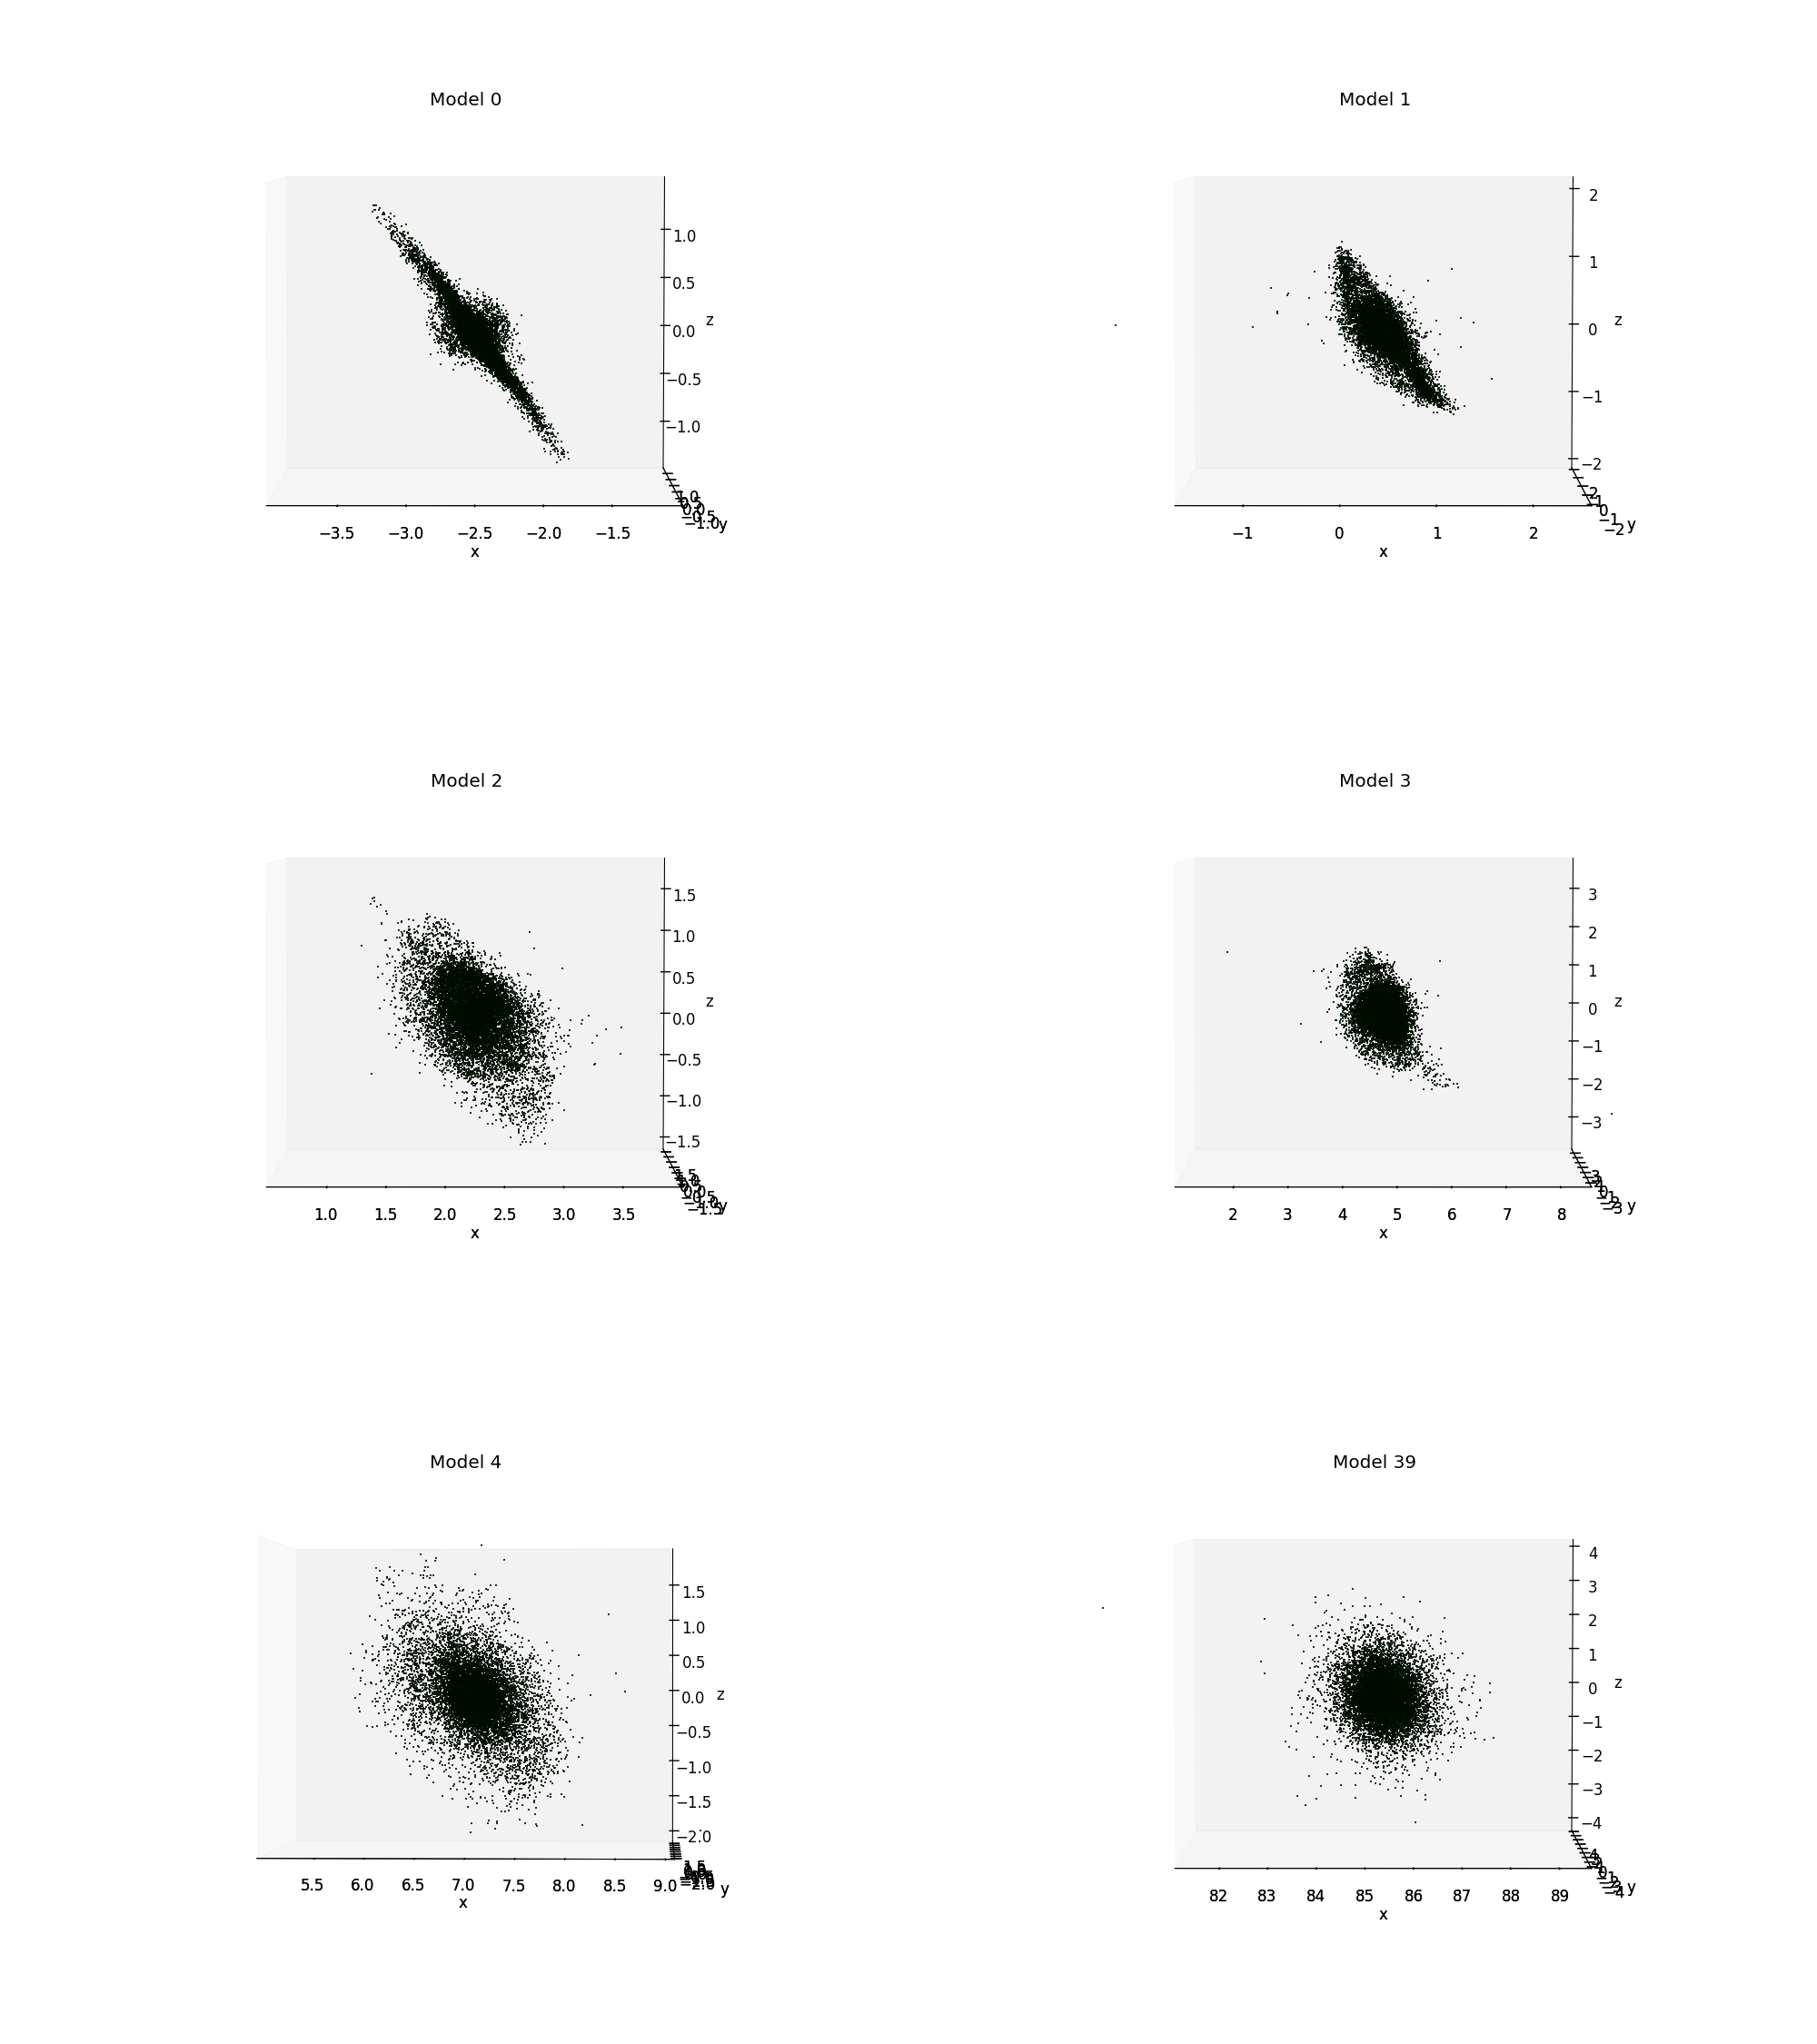
\includegraphics[scale=0.2]{60deg-m-c2y.png}
 \caption{\emph{ ángulo = 60 grados, el objeto con disco visto en la dirección oy(solo parte luminosa) modelo 0,1,2,3,4,39 }}
\end{figure}

\begin{figure}[!ht]
 \centering
 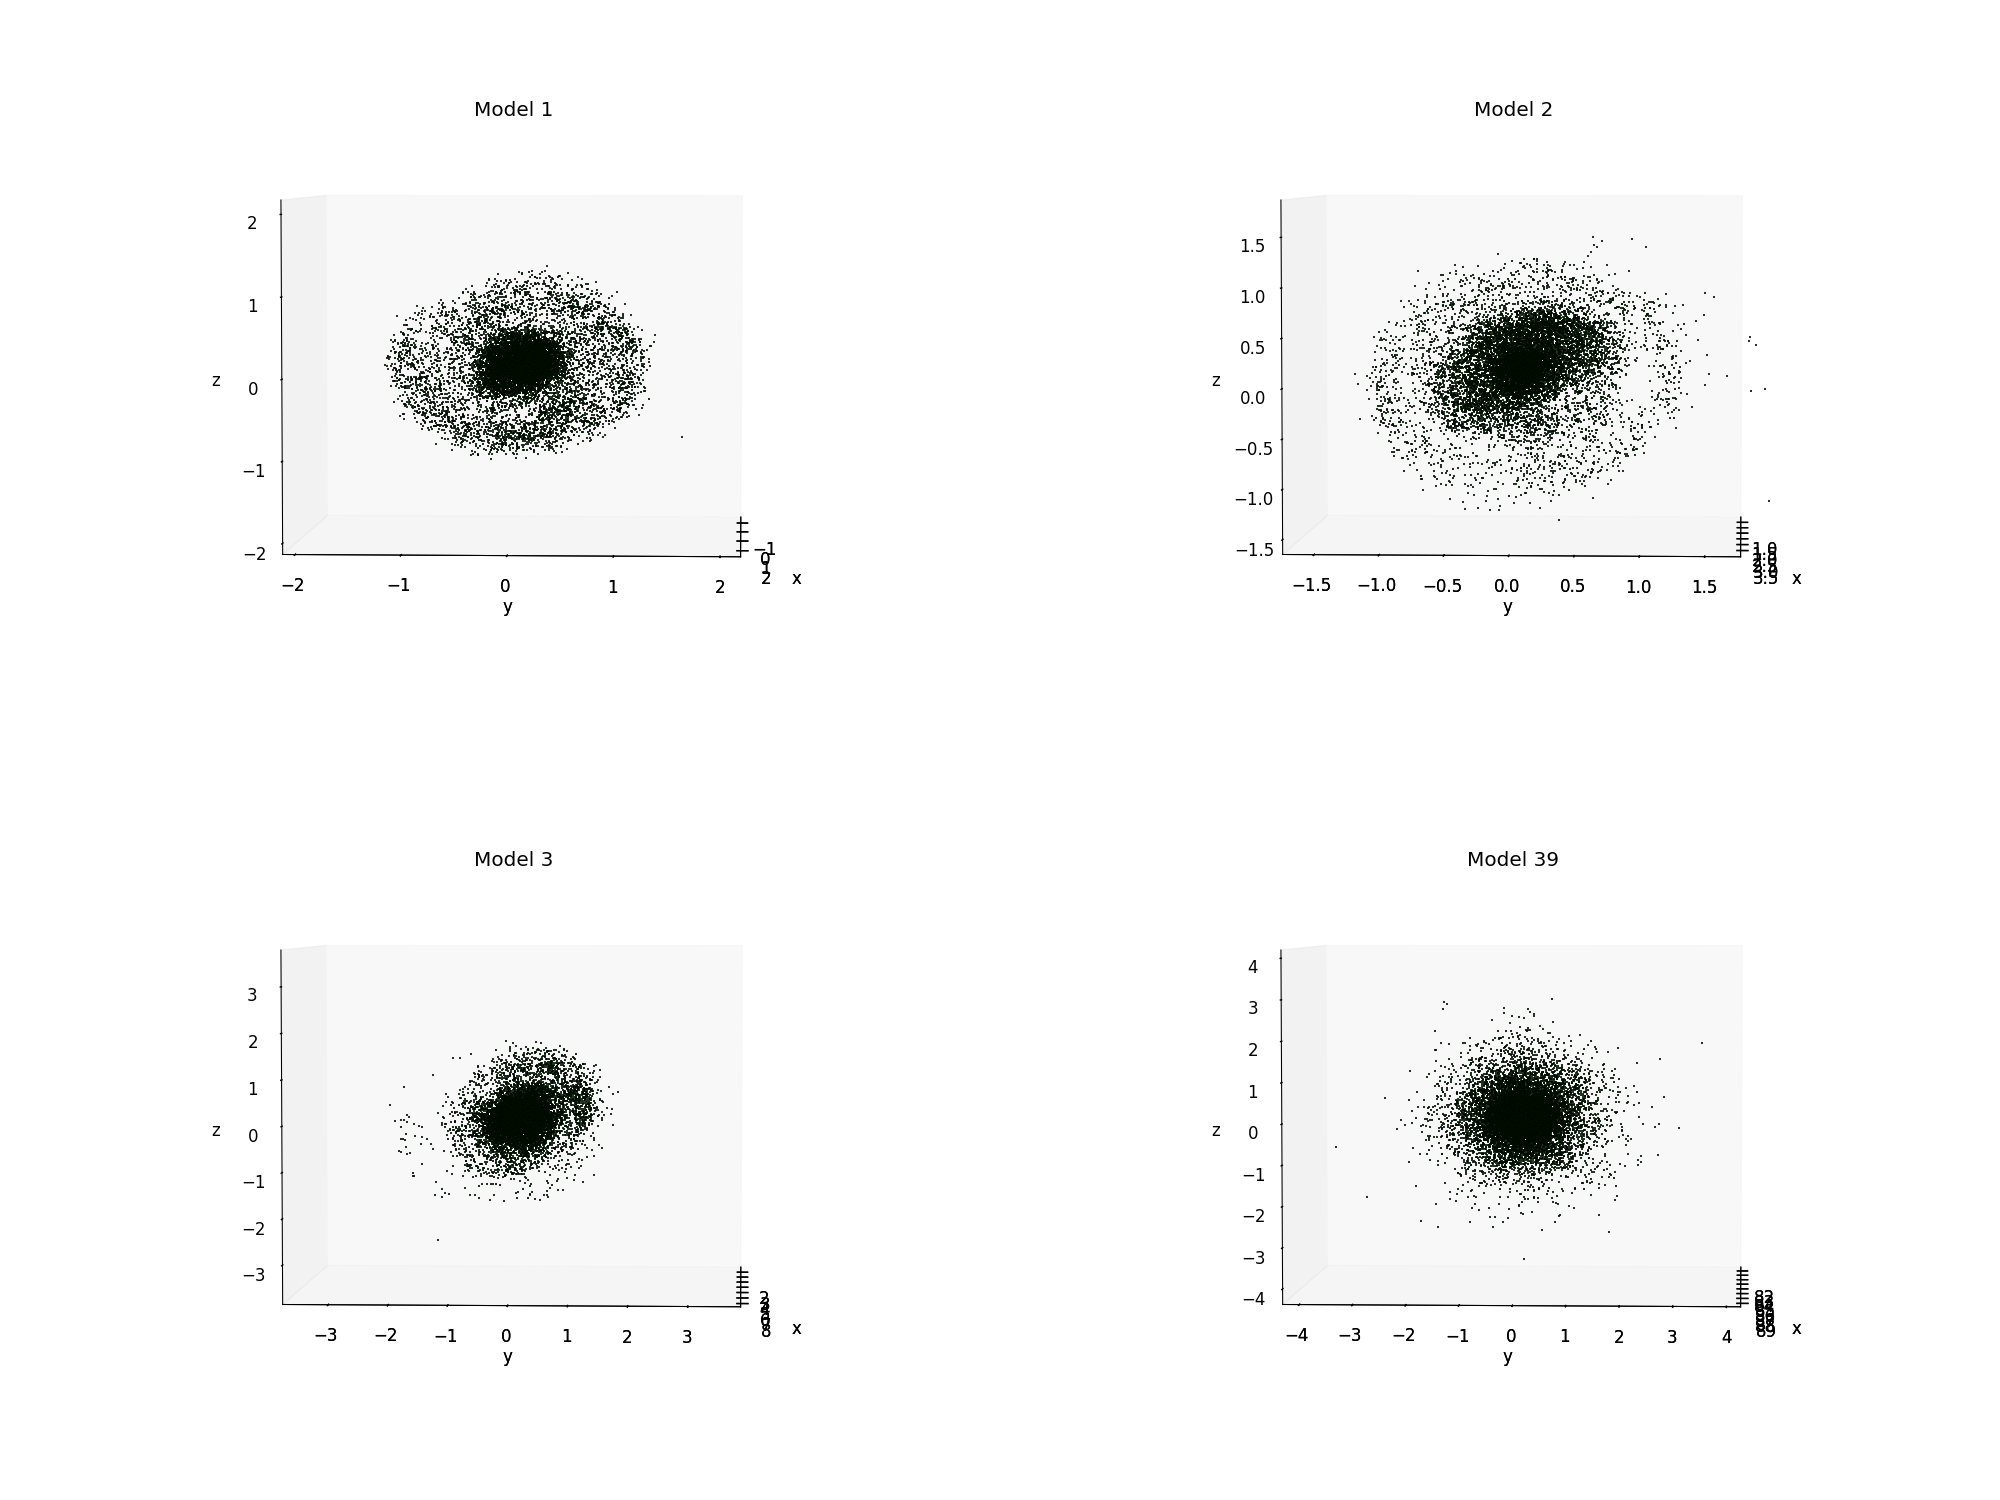
\includegraphics[scale=0.2]{60deg-m-c2.png}
 \caption{\emph{ ángulo = 60 grados, el objeto con disco visto en la dirección ox(solo parte luminosa) modelo 1,2,3,39 }}
\end{figure}

\begin{figure}[!ht]
 \centering
 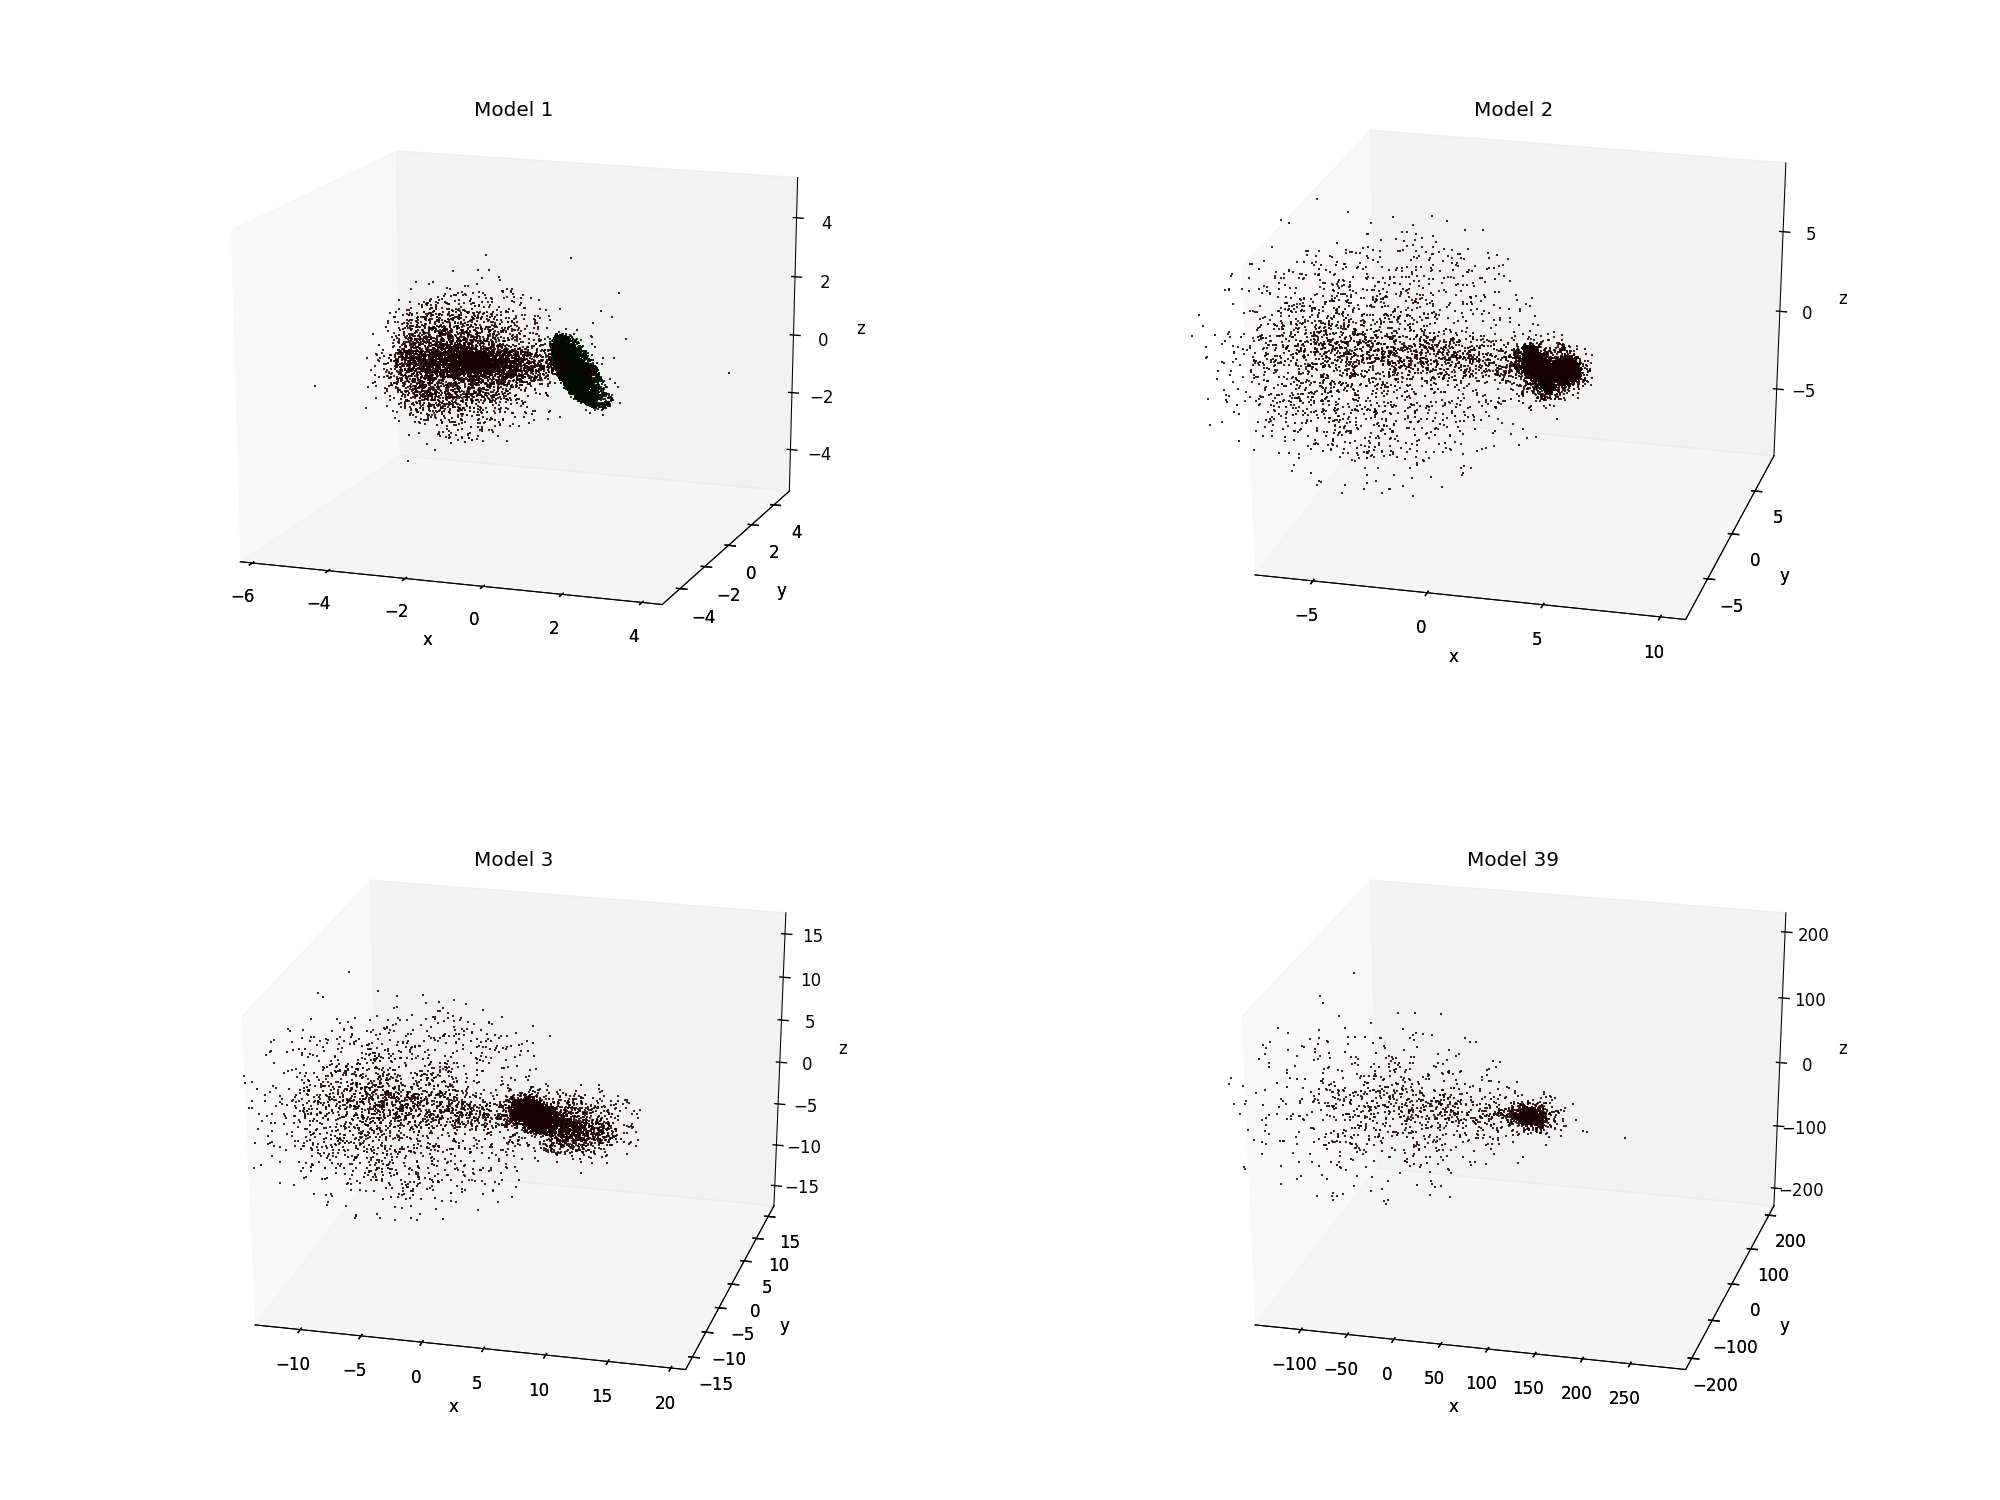
\includegraphics[scale=0.2]{240deg-m.png}
 \caption{\emph{ ángulo = 240 grados, los 2 objetos(solo parte luminosa) modelo 1,2,3,39 }}
\end{figure}

\begin{figure}[!ht]
 \centering
 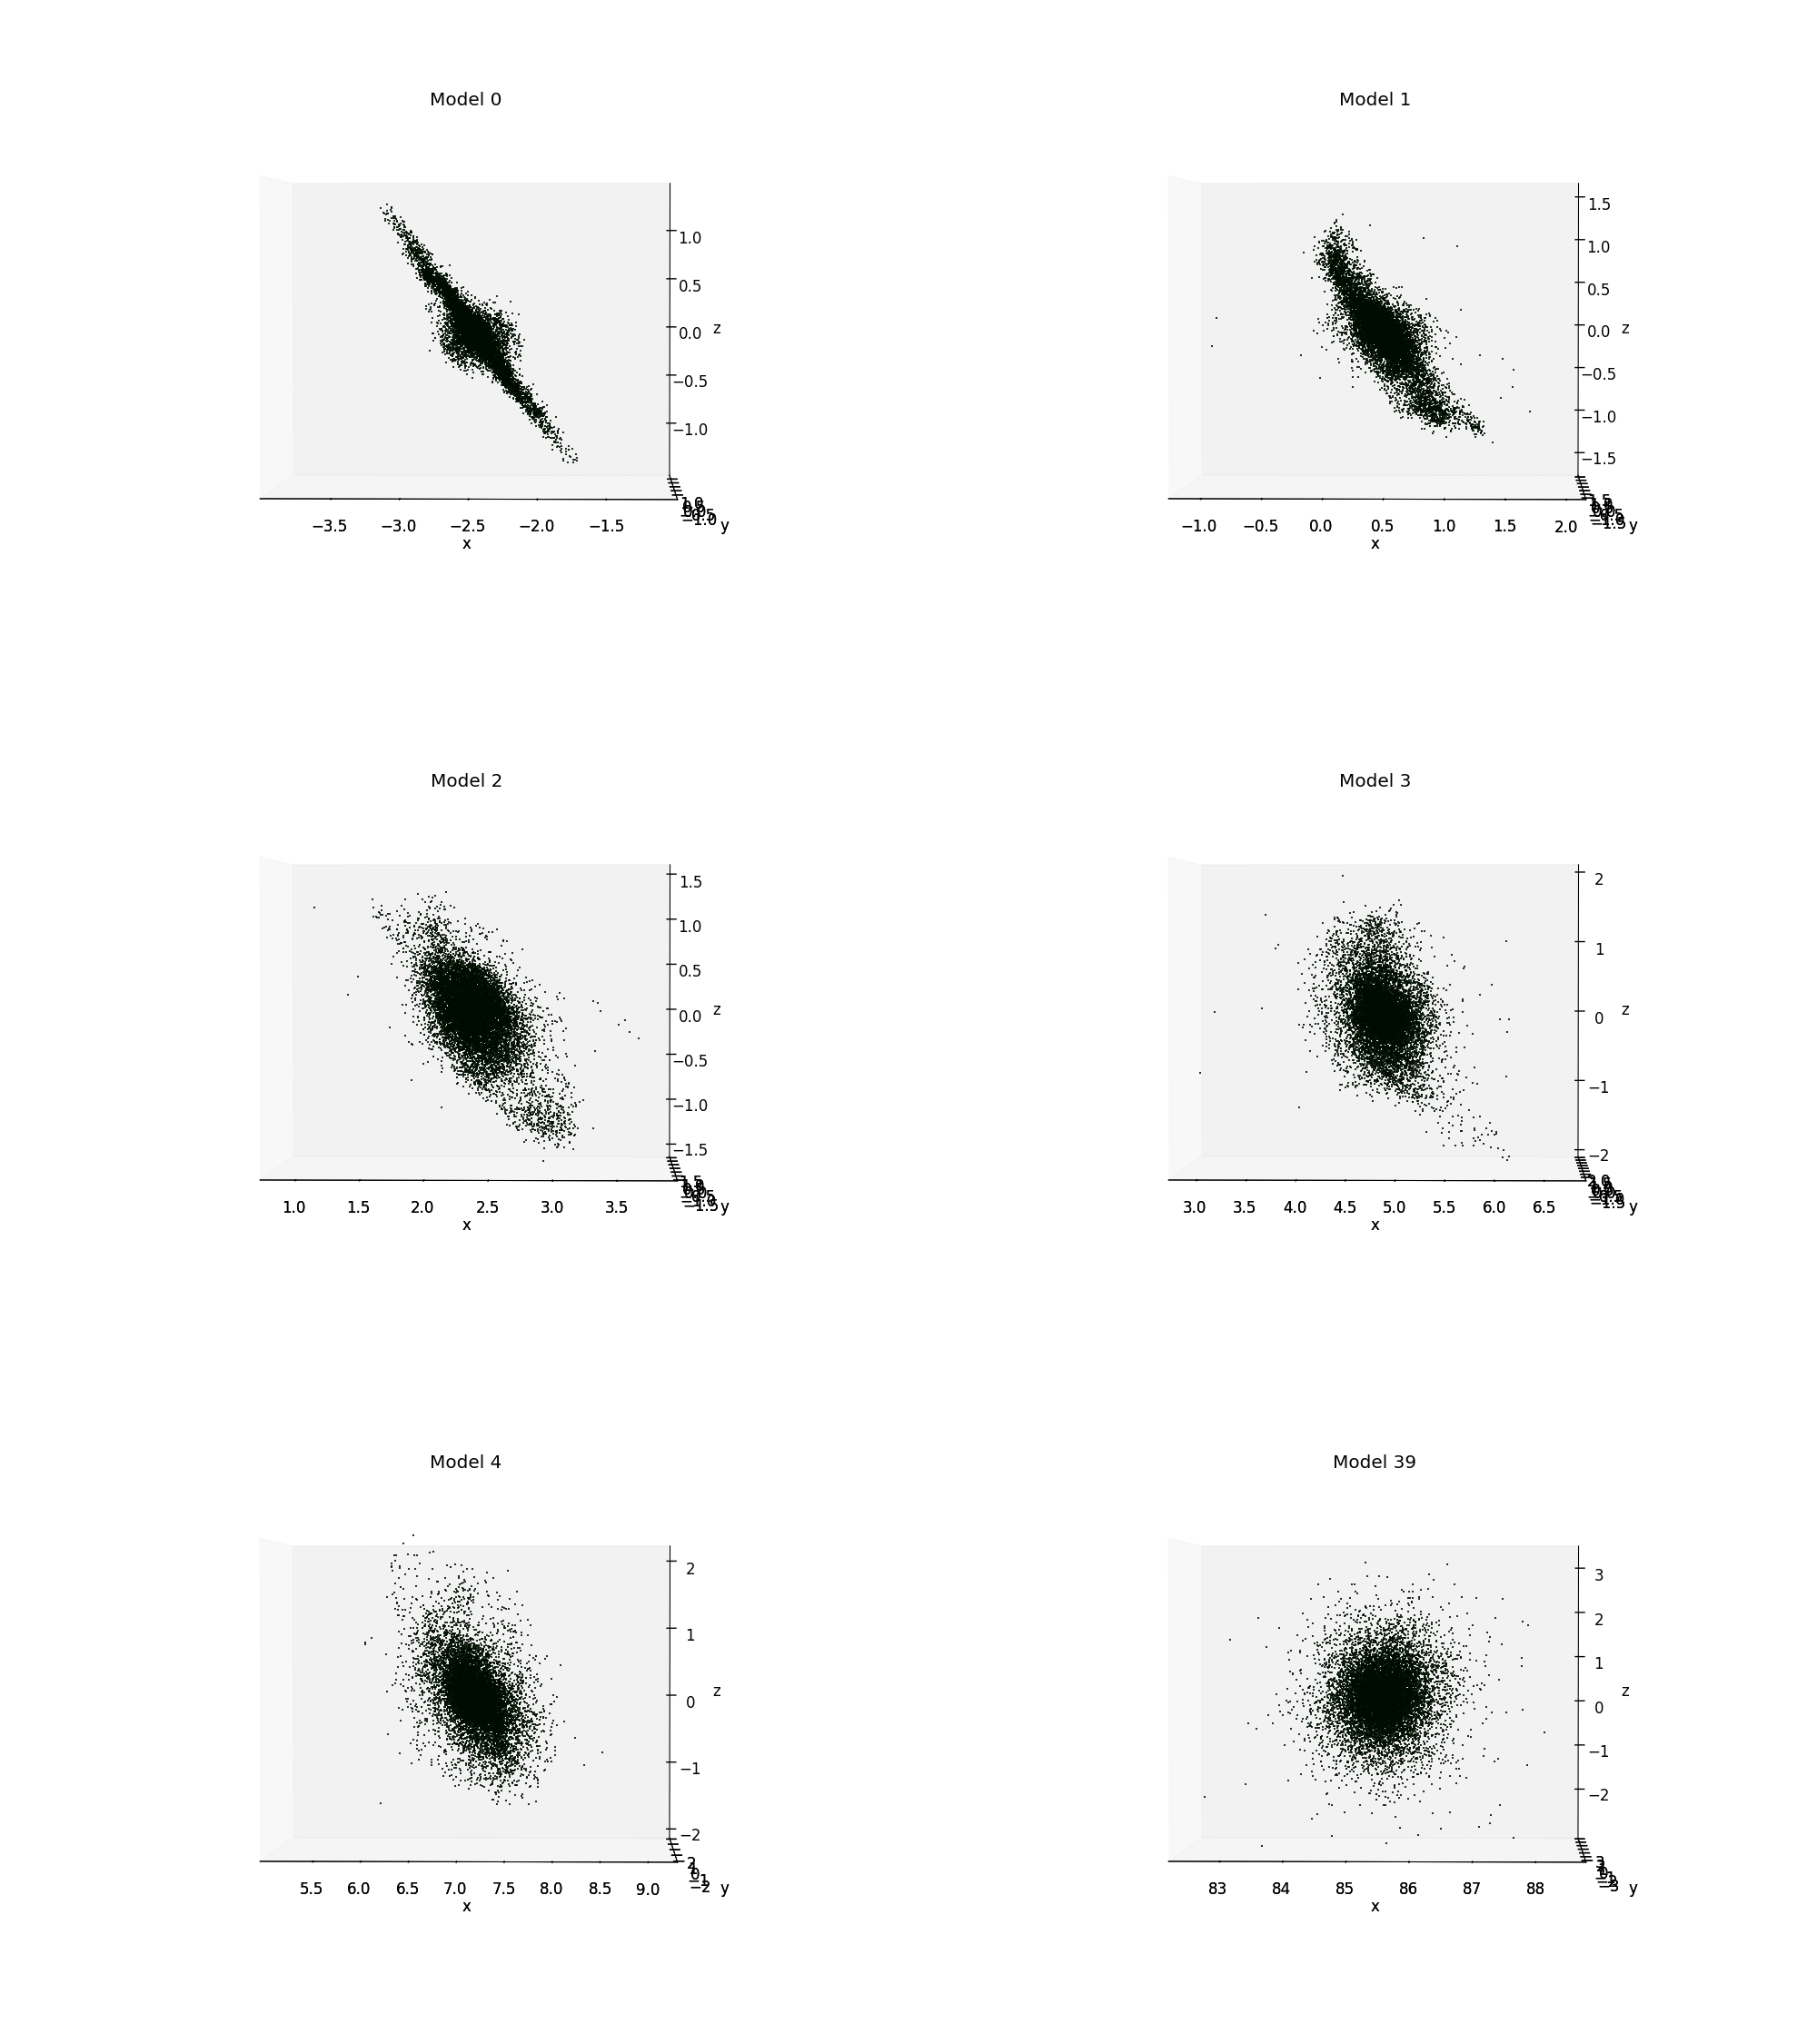
\includegraphics[scale=0.2]{240deg-m-c2y.png}
 \caption{\emph{ ángulo = 240 grados, el objeto con disco visto en la dirección oy(solo parte luminosa) modelo 0,1,2,3,4,39 }}
\end{figure}

\begin{figure}[!ht]
 \centering
 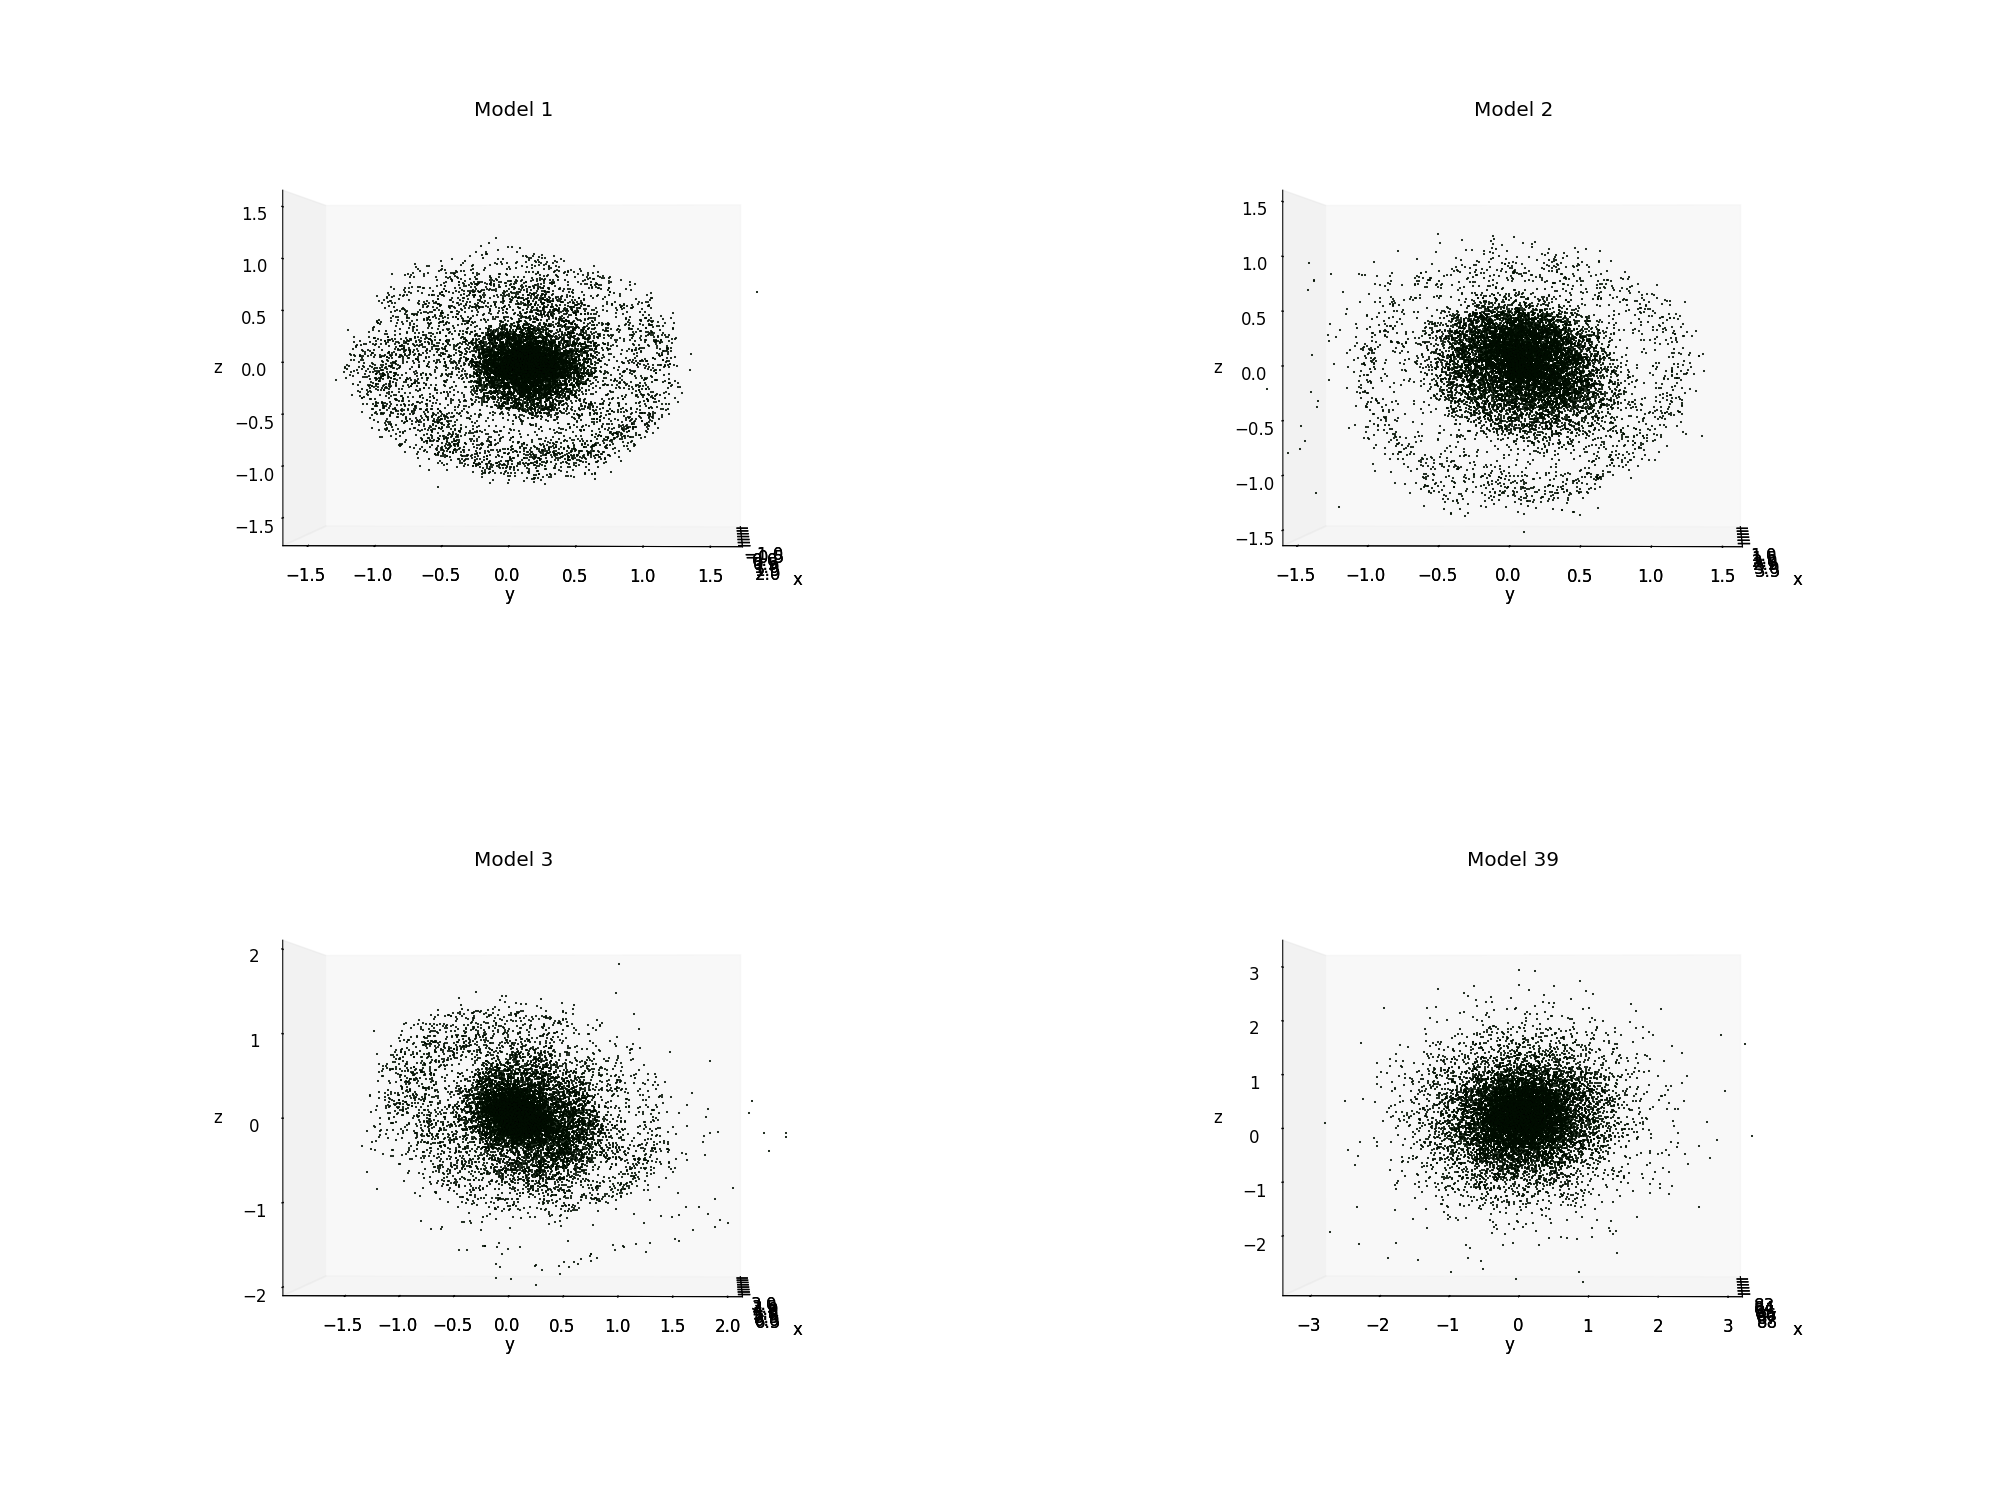
\includegraphics[scale=0.2]{240deg-m-c2.png}
 \caption{\emph{ ángulo = 240 grados, el objeto con disco visto en la dirección ox(solo parte luminosa) modelo 1,2,3,39 }}
\end{figure}




\begin{figure}[!ht]
 \centering
 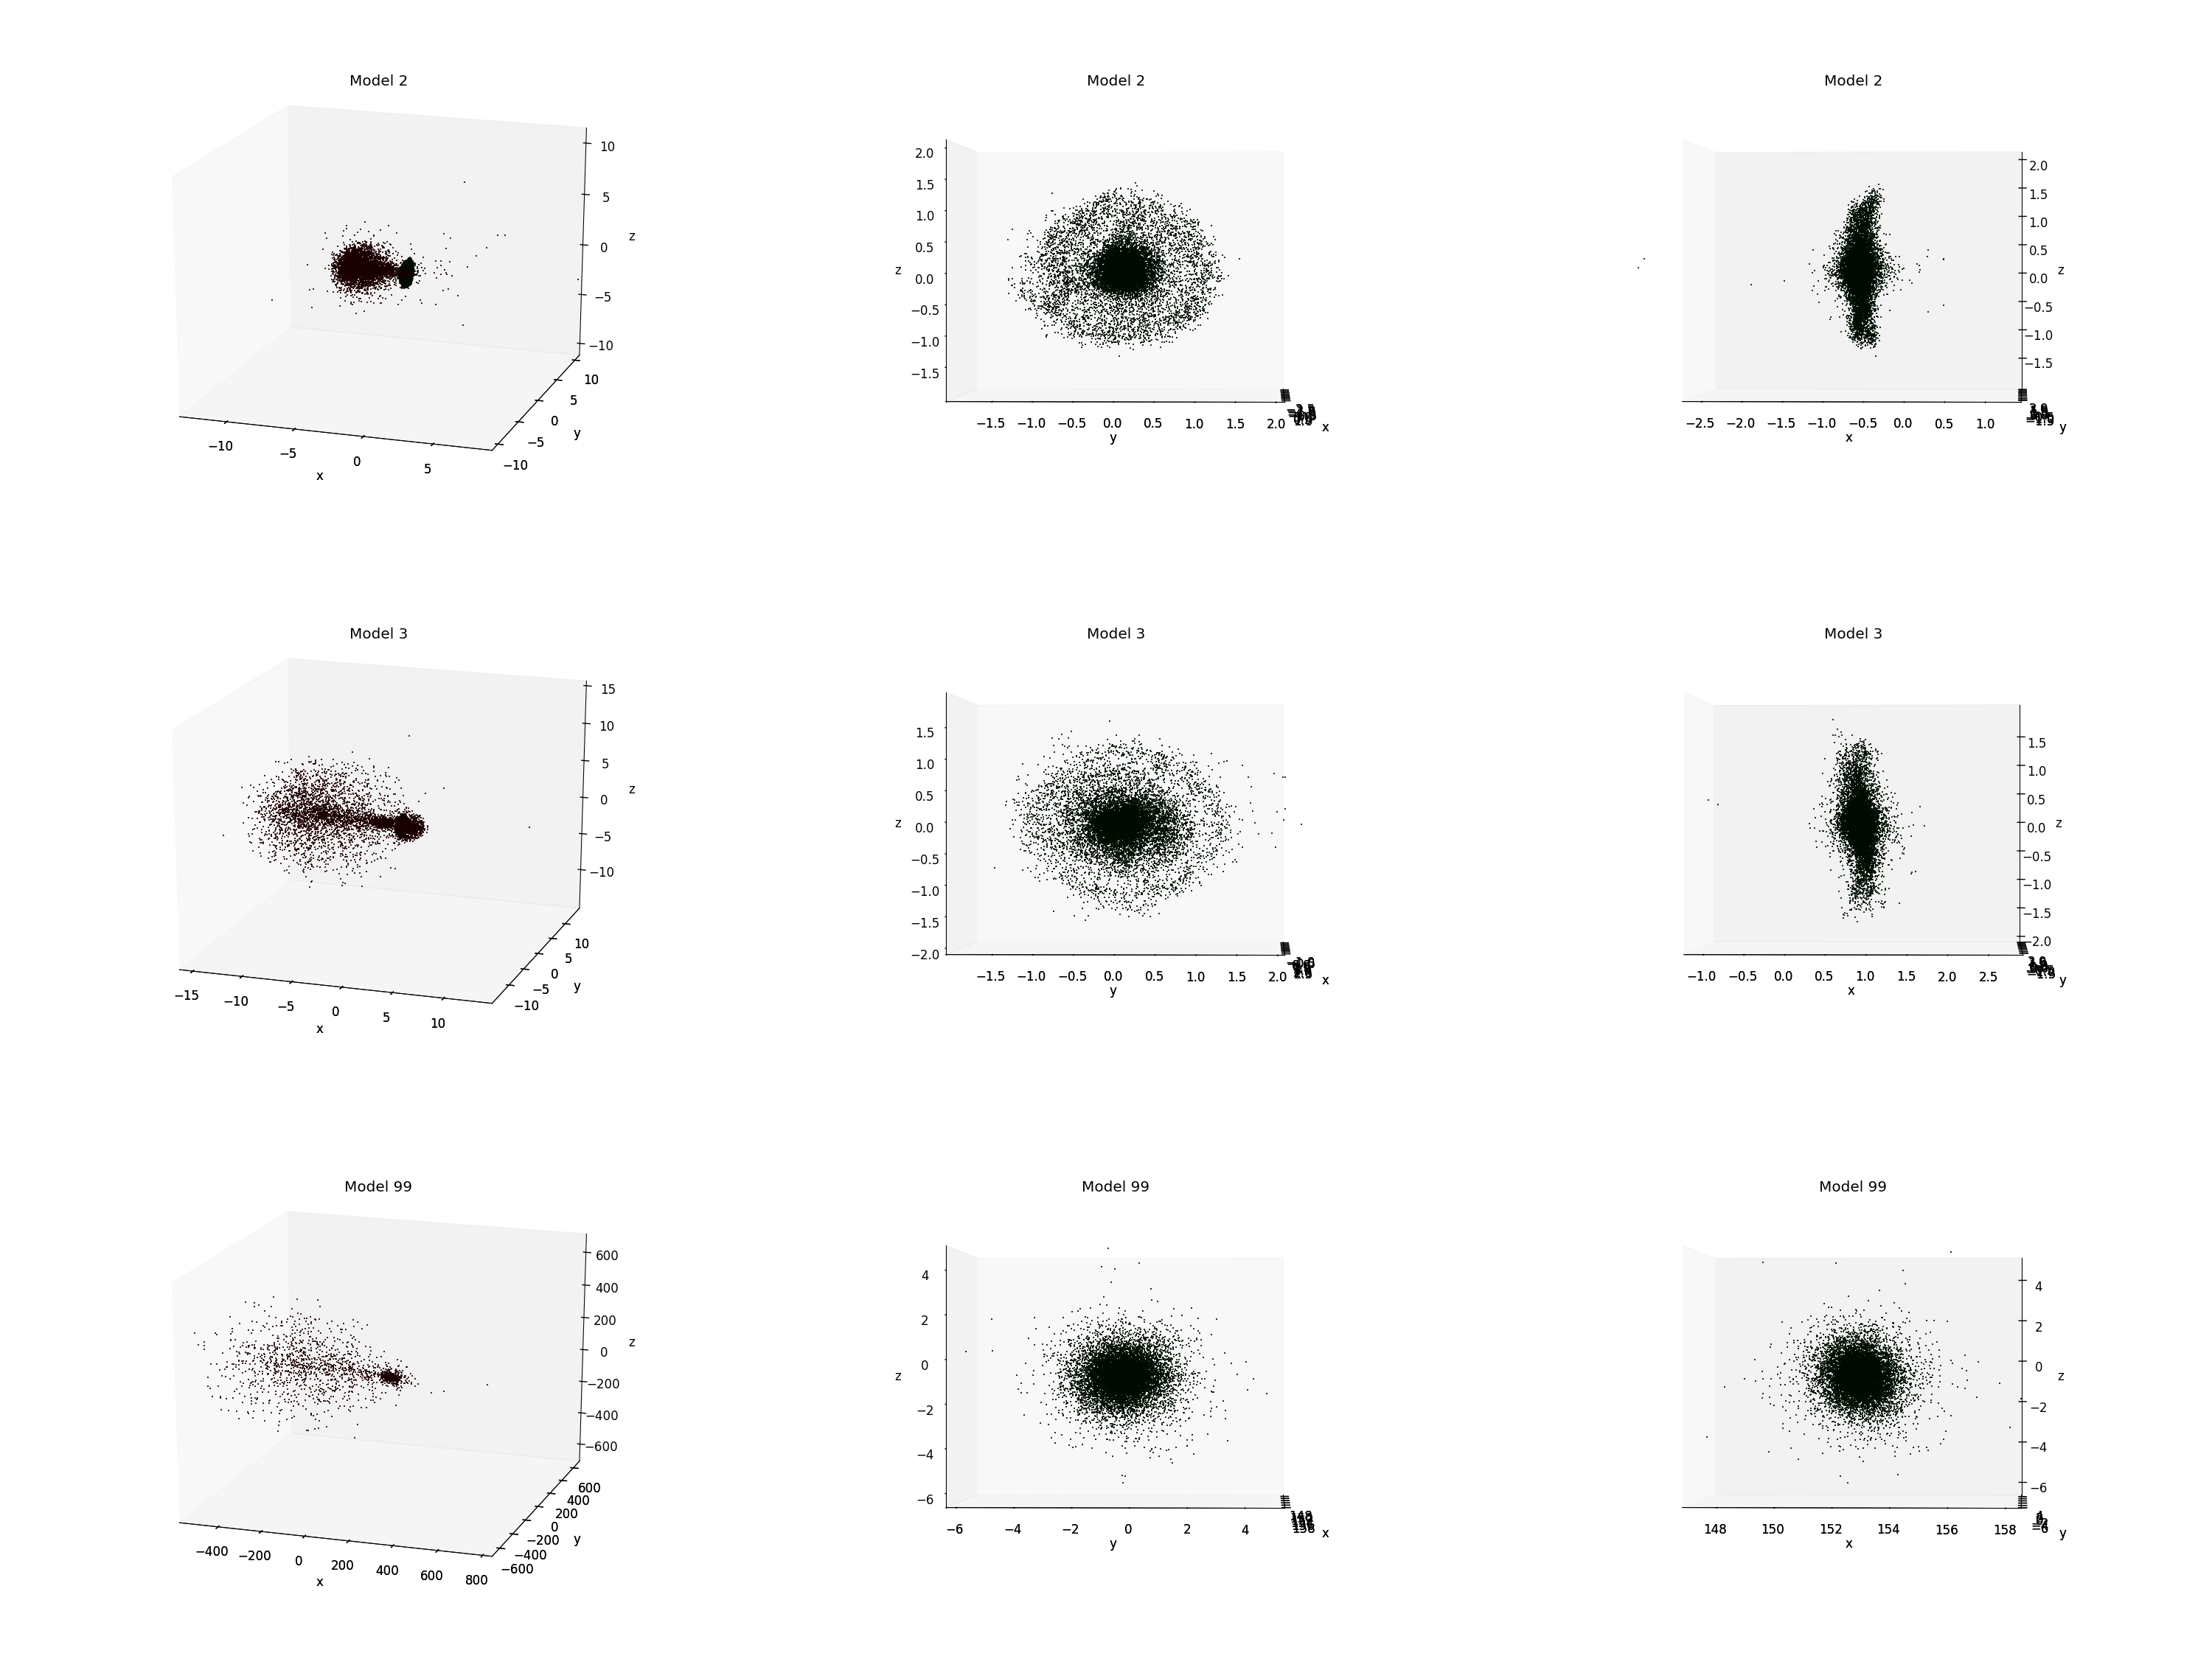
\includegraphics[scale=0.2]{sep10.png}
 \caption{\emph{ Separación = 10 , ángulo = 90 grados, el objeto con disco visto en la dirección ox(solo parte luminosa) modelo 2,3,99 }}
\end{figure}



\end{document}
